% ACC 2027 / PaperPlaza official class. ieeeconf.cls MUST sit in the project
% root next to this file - Overleaf does not search subfolders for .cls.
\documentclass[letterpaper, 10 pt, conference]{ieeeconf}

\IEEEoverridecommandlockouts   % required before \thanks in ieeeconf
\overrideIEEEmargins           % required to meet the ACC printer margins

\usepackage{amsmath,amssymb,bm}
\let\proof\relax
\let\endproof\relax
\usepackage{amsthm} % for theorem/proof environments
\newtheorem{theorem}{Theorem}
% for theorem/proof environments
\usepackage{booktabs,array,cite}
\usepackage{graphicx}
\usepackage[hidelinks]{hyperref}
% Figures live under figures/..., so keep that on the graphics path.
\graphicspath{{figures/}{figures/disturbance/}{../experiments/nengo_nef_replication_2026-08-29/results/plots/}}

% [v6] TikZ support for the architecture figures.
\usepackage{tikz}
\usepackage{verbatim}
\usetikzlibrary{arrows.meta,positioning,fit,backgrounds,calc}
% Architecture drawing helpers live in architectures/tikz/.
% Shared TikZ style for all architecture figures. Grayscale-safe.
\tikzset{
  blk/.style   ={draw,rounded corners=2pt,align=center,font=\footnotesize,
                 minimum height=8mm,inner sep=3pt,fill=white},
  clas/.style  ={blk,fill=black!4},
  neuro/.style ={blk,fill=black!12,very thick},
  plant/.style ={blk,fill=black!20},
  meas/.style  ={blk,dashed},
  sum/.style   ={draw,circle,inner sep=0pt,minimum size=4.5mm,font=\scriptsize},
  sig/.style   ={-{Latex[length=2mm]},thick},
  sigd/.style  ={-{Latex[length=2mm]},thick,dashed},
  lbl/.style   ={font=\scriptsize,inner sep=1.5pt,fill=white},
  grp/.style   ={draw,dashed,rounded corners=3pt,inner sep=6pt},
  note/.style   ={font=\scriptsize\itshape,align=left},
}


\newcommand{\R}{\mathbb R}
\newcommand{\T}{^{\mathsf T}}
\newcommand{\sat}{\operatorname{sat}}
\newcommand{\clip}{\operatorname{clip}}
\newcommand{\sgnp}{\operatorname{sgn}_{+}}
\newtheorem{proposition}{Proposition}
\newtheorem{remark}{Remark}

% [v7] Title now names the mechanism and the learning, and claims the
% controlled study rather than architectural novelty.
\title{\LARGE \bf Online PES Decoder Learning in Neuromorphic Residual Control of UAV Quaternion Tracking}

% ACC/PaperPlaza template author format (ieeeconf.cls does not support IEEEtran blocks).
\author{Gandhi Contreras$^{1}$, Steven Sandoval$^{1}$, and Luis Rodolfo Garcia Carrillo$^{2}$%
\thanks{$^{1}$New Mexico State University (NMSU), Las Cruces, NM, USA.}%
\thanks{$^{2}$ Space Vehicles Directorate, Air Force Research Laboratory (AFRL), Kirtland Air Force Base (KAFB), Albuquerque, NM 87108.
    Email: {\tt\small luis\_rodolfo.garcia\_carrillo@afrl.af.mil}}%
}

\begin{document}
\maketitle

% NOTE: The official ACC/PaperPlaza template often suppresses page numbers for
% submission. If you need page numbers for internal review, use `plain`.
\pagestyle{plain}
\thispagestyle{plain}

% [v7] Rewritten: leads with the mechanism and the result; scope limits kept
% but stated once rather than after every claim.
%We present a compact neuromorphic residual controller for quaternion attitude tracking with bounded actuator commands. A fixed quaternion PD baseline is augmented by six paired coupled membrane--gate (CMG) units: continuous, non-spiking, conductance-based neurons whose gate-derived activities form a nonlinear basis. Eighteen decoder weights adapt online via prescribed error sensitivity (PES), and the bounded residual is \emph{added} to the saturated baseline so the baseline is recovered exactly at zero authority. We give bounds on internal states, command deviation, and projected decoder weights, and we isolate three commonly conflated mechanisms: intrinsic conductance modulation, decoder learning, and residual authority.
%In ten matched 45-s MuJoCo cases spanning five missions on Skydio X2 and Crazyflie~2.0 models (the latter completed with an explicit four-rotor interface), CMG--PES reduces mean quaternion-angle error by $17.3$--$60.6\%$ relative to PD while respecting actuator limits (nonzero bound occupancy only in brief Hardstep intervals). Direct and Nengo implementations agree to $2.013\times10^{-6}$ relative mean error. In the tested gain regime, most of the improvement is carried by online decoder adaptation; toggling conductance modulation is numerically indistinguishable. A benchmark against LIF, ALIF, Izhikevich, and LIFRate bases shows the same hierarchy and exposes an effort--accuracy tradeoff: families that match CMG--PES on error spend several times its residual authority to do so. Noise reruns keep the reduction range at $18.1$--$55.8\%$ with seed standard deviation below $0.031\%$, and an intermittent-disturbance study shows learned corrections reused across episodes. Results are in simulation and establish boundedness, not closed-loop stability.

\begin{abstract}
Online neuromorphic residual control can augment a classical attitude controller under abrupt missions or unforeseen disturbances without changing its feedback gains or actuator interface. We present six continuous coupled membrane-gate (CMG) units and eighteen decoder weights adapted by prescribed error sensitivity (PES), adding a bounded correction to the saturated quaternion proportional-derivative (PD) torque request before rotor-force allocation. Across ten matched 45-second MuJoCo cases on the Skydio X2 and a Crazyflie~2 derived model, mean quaternion-angle error decreases by 17.3--60.6\%, including approximately 53--57\% reductions on the Full3 and Hard45 multi-axis tracking missions. Direct and Nengo implementations agree closely. Benchmarks against LIF, ALIF, Izhikevich, and LIFRate neuron models expose an effort-accuracy tradeoff: CMG--PES attains better tracking with substantially lower realized residual effort. Under synthetic measurement noise, the error reductions persist, and learned corrections are reused across repeated disturbances. Overall, PD provides a nominal, interpretable reference, while the online residual adds bounded, revocable adaptation that improves robustness to disturbances and noisy measurements.
\end{abstract}

\section{Introduction}

Learning-based augmentation can retain classical feedback while adapting a correction that is difficult to specify \emph{a priori}. We study a bounded torque residual for quaternion attitude tracking of an unmanned aerial vehicle (UAV) with individual rotor-force saturation. The question is whether a small stateful basis improves a fixed PD controller, and whether any improvement comes from its neuron dynamics, decoder learning, or correction magnitude. Bounded authority makes the learning layer switchable; it does not by itself ensure stability or safety.

Prior work includes residual robot learning \cite{johannink2019}, geometric $\mathcal L_1$ quadrotor augmentation with performance guarantees \cite{wu2025l1quad}, and proportional--integral--derivative (PID) attitude control augmented with a proximal policy optimization (PPO) residual \cite{li2027hpappo}.
%
Neuromorphic control offers a complementary implementation approach: Nengo supports the Neural Engineering Framework (NEF) and online decoder learning \cite{bekolay2014nengo}, most often through the prescribed error sensitivity (PES) rule, an established local, online error-driven update \cite{voelker2015pes}. PES-based adaptive control has been demonstrated on manipulators \cite{dewolf2016arm,dewolf2020nengo}, and in a Nengo spiking PID controller for a free-flying UAV \cite{olivares2026selftuning}.  
Building on that line, our focus is a continuous membrane-gate basis for a bounded quaternion-torque residual, with a fixed classical controller and adaptation confined to its decoder.

We augment a quaternion PD baseline with a compact neuromorphic residual architecture based on coupled conductance-based membrane-gate (CMG) units and PES decoder learning. The paper's contributions are:
\begin{enumerate}
    \item a code-aligned CMG--PES architecture with paired currents, explicit encoding, state-update, and decoder/readout equations, and a fully specified actuator interface (Fig.~\ref{fig:arch});
    \item proofs of internal-state, command-deviation, and weight boundedness, with exact recovery of the PD baseline at zero residual authority;
    \item a controlled ablation that separates conductance modulation, decoder learning, and output authority, and identifies which mechanism is primarily responsible for the tracking-error reduction; and
    \item robustness evidence that the reduction survives realistic measurement noise, together with a hold-equilibrium study in which the learned correction is reused across repeated disturbance episodes rather than relearned.
\end{enumerate}

  %\item a matched five-mission, two-model study in which the direct and Nengo realizations agree to within $2.013\times10^{-6}$ in the maximum relative mean quaternion-angle tracking error difference across the ten missions;

The CMG unit couples a leaky membrane to a gating state that modulates its effective conductance, linking LIF-like membrane integration with Hodgkin--Huxley inspired gating dynamics. Although related operating regimes can support spike-like responses, the present controller deliberately exploits the continuous, non-spiking membrane-gate trajectory, which provides a compact set of stateful temporal features for the residual.
The present implementation is digital; the same temporal-feature mechanism holds regardless of computing platform, and no neuromorphic-hardware energy advantage is claimed.

The remainder of the paper is organized as follows. Section~\ref{sec:problem} defines the attitude-tracking problem, notation, and actuator interface. Section~\ref{sec:architecture} presents the CMG--PES residual architecture, state dynamics, and learning rule. Section~\ref{sec:analysis} establishes boundedness properties. Section~\ref{sec:results} reports the simulation study, ablations, and benchmarks, including noise and repeated-disturbance experiments. Section~\ref{sec:conclusion} concludes and discusses limitations and future work.

% [v6] Architecture overview (TikZ source under architectures/tikz/).

\begin{figure*}
    \centering
    % Trim bottom whitespace in the standalone PDF so the caption sits closer.
    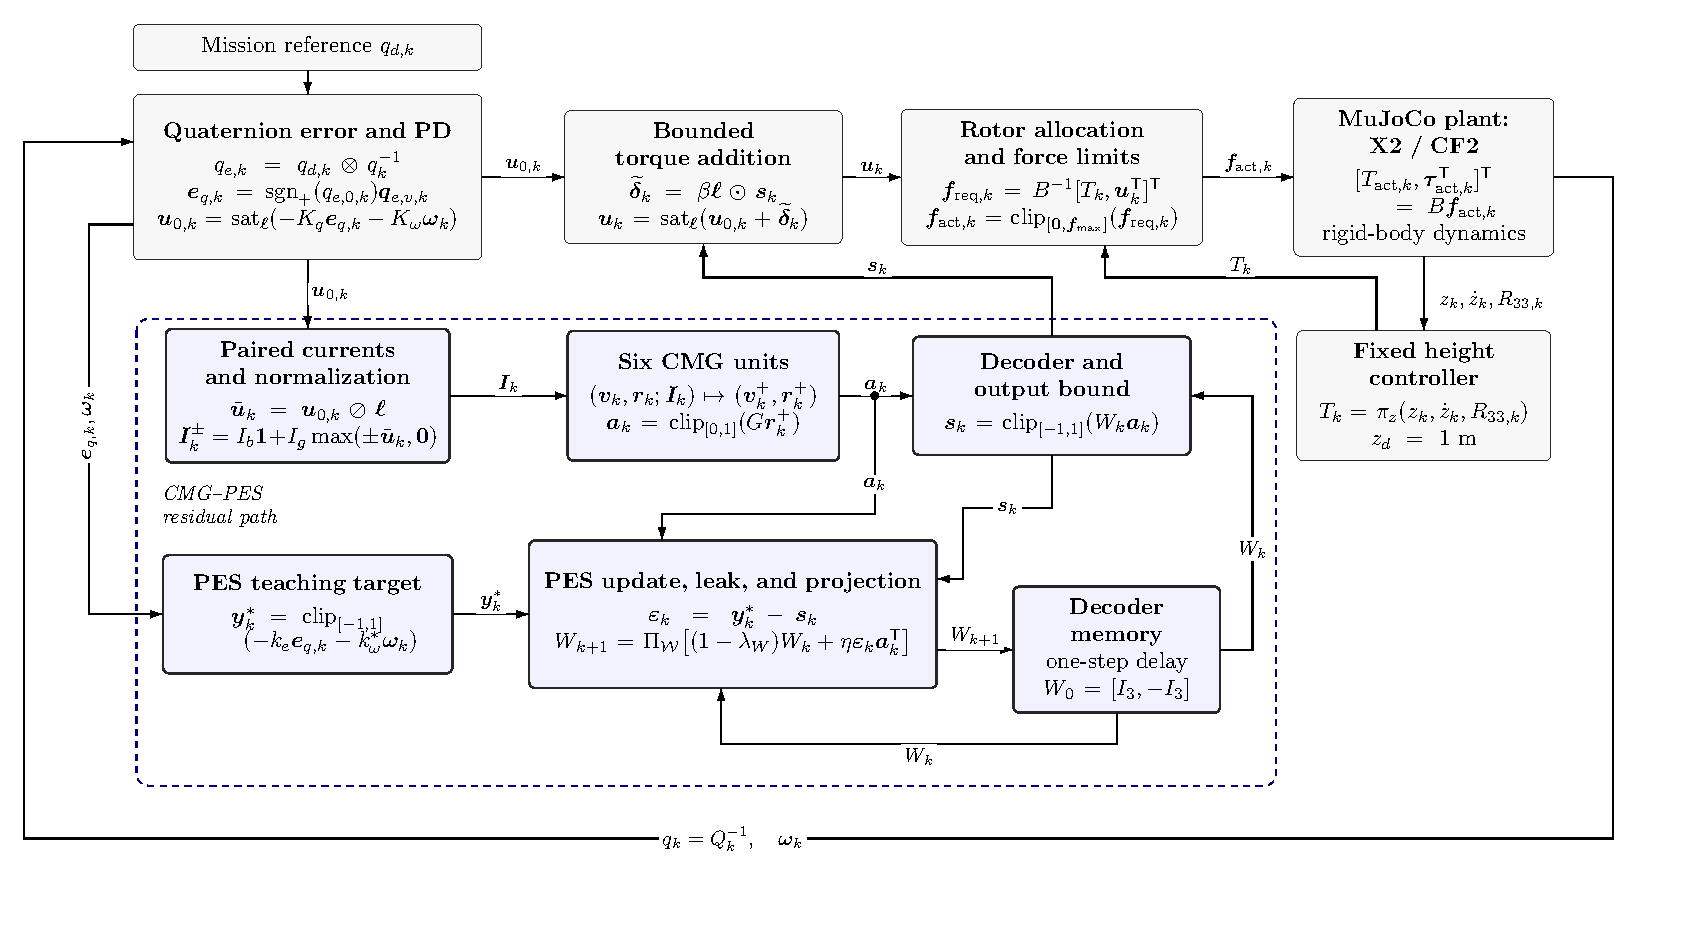
\includegraphics[width=\textwidth,trim=0 10mm 0 0,clip]{architectures/architecture_standalone.pdf}
    \caption{Online PES decoder learning CMG-PES Neuromorphic Residual Control architecture}
    \label{fig:arch}
\end{figure*}

\begin{comment}
\begin{figure*}[t]

\centering
\resizebox{\textwidth}{!}{% A2p -- paper variant of A2: same diagram, annotation note removed
% (it belongs in the caption). Intended for a two-column figure* at
% \textwidth; no \resizebox needed at 10pt.
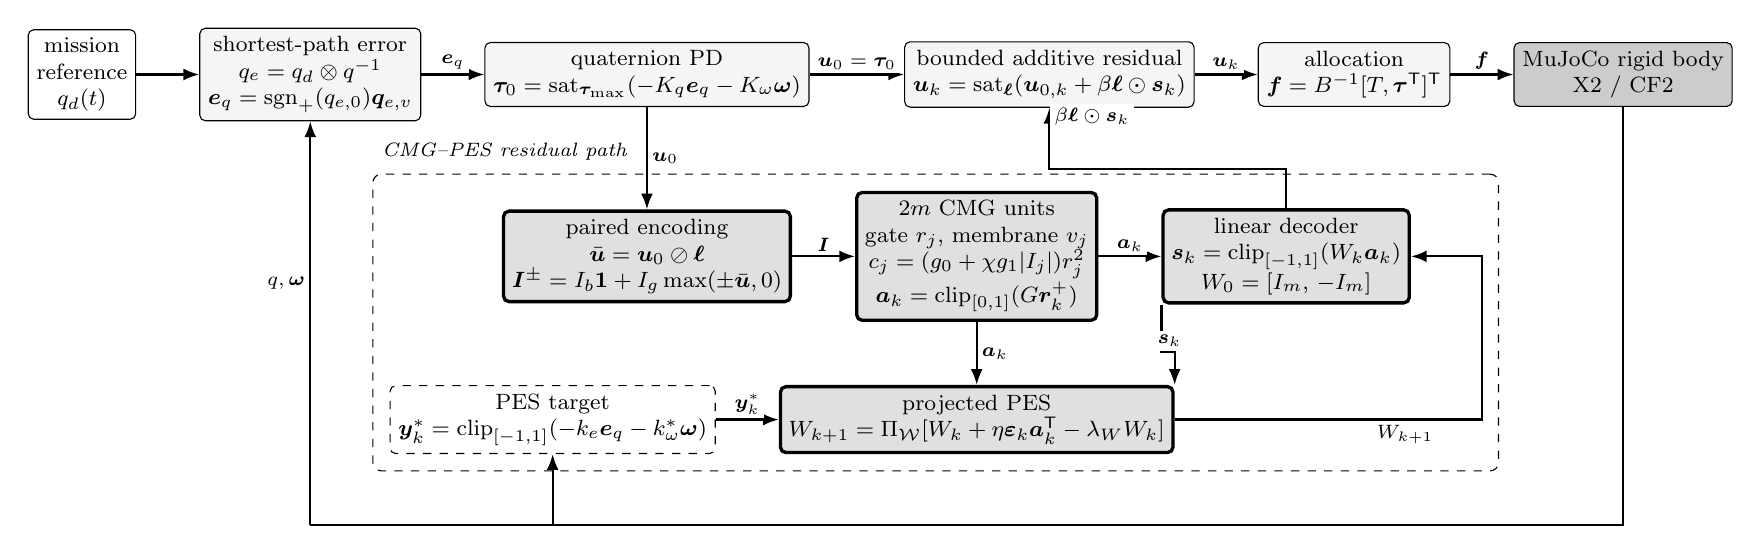
\begin{tikzpicture}[node distance=6mm and 8mm]
  \node[blk]                    (ref)  {mission\\reference\\$q_d(t)$};
  \node[clas,right=of ref]      (err)  {shortest-path error\\
                                        $q_e=q_d\otimes q^{-1}$\\
                                        $\bm e_q=\sgnp(q_{e,0})\bm q_{e,v}$};
  \node[clas,right=of err]      (pd)   {quaternion PD\\
                                        $\bm\tau_0=\sat_{\bm\tau_{\max}}(-K_q\bm e_q-K_\omega\bm\omega)$};
  \node[clas,right=12mm of pd]  (res)  {bounded additive residual\\
                                        $\bm u_k=\sat_{\bm\ell}(\bm u_{0,k}+\beta\bm\ell\odot\bm s_k)$};
  \node[clas,right=of res]      (alc)  {allocation\\$\bm f=B^{-1}[T,\bm\tau\T]\T$};
  \node[plant,right=of alc]     (plt)  {MuJoCo rigid body\\X2 / CF2};

  \node[neuro,below=13mm of pd] (enc)  {paired encoding\\
                                        $\bar{\bm u}=\bm u_0\oslash\bm\ell$\\
                                        $\bm I^{\pm}=I_b\bm 1+I_g\max(\pm\bar{\bm u},0)$};
  \node[neuro,right=of enc]     (cmg)  {$2m$ CMG units\\
                                        gate $r_j$, membrane $v_j$\\
                                        $c_j=(g_0+\chi g_1|I_j|)r_j^2$\\
                                        $\bm a_k=\clip_{[0,1]}(G\bm r_k^{+})$};
  \node[neuro,right=of cmg]     (dec)  {linear decoder\\
                                        $\bm s_k=\clip_{[-1,1]}(W_k\bm a_k)$\\
                                        $W_0=[I_m,\,-I_m]$};
  \node[neuro,below=8mm of cmg](pes)  {projected PES\\
                                        $W_{k+1}=\Pi_{\mathcal W}[W_k+\eta\bm\varepsilon_k\bm a_k\T-\lambda_W W_k]$};
  \node[meas,left=of pes]       (tgt)  {PES target\\
                                        $\bm y^*_k=\clip_{[-1,1]}(-k_e\bm e_q-k^*_\omega\bm\omega)$};

  \draw[sig] (ref) -- (err);
  \draw[sig] (err) -- node[lbl,above]{$\bm e_q$} (pd);
  \draw[sig] (pd)  -- node[lbl,above]{$\bm u_0=\bm\tau_0$} (res);
  \draw[sig] (res) -- node[lbl,above]{$\bm u_k$} (alc);
  \draw[sig] (alc) -- node[lbl,above]{$\bm f$} (plt);

  \draw[sig] (pd.south) -- node[lbl,right]{$\bm u_0$} (enc.north);
  \draw[sig] (enc) -- node[lbl,above]{$\bm I$} (cmg);
  \draw[sig] (cmg) -- node[lbl,above]{$\bm a_k$} (dec);
  \draw[sig] (dec.north) -- ++(0,5mm) -| node[lbl,pos=.93,right]{$\beta\bm\ell\odot\bm s_k$} (res.south);
  \draw[sig] (cmg.south) -- node[lbl,right]{$\bm a_k$} (pes.north);
  \draw[sig] (tgt) -- node[lbl,above]{$\bm y^*_k$} (pes);
  \draw[sig] (dec.south west) -- ++(0,-6mm) -| node[lbl,pos=.3,above]{$\bm s_k$} (pes.north east);
  \coordinate (wx) at ($(dec.east)+(9mm,0)$);
  \draw[sig] (pes.east) -- node[lbl,pos=.75,below]{$W_{k+1}$} (pes.east-|wx) -- (wx) -- (dec.east);

  \coordinate (busy) at ($(pes.south)+(0,-9mm)$);
  \draw[thick] (plt.south) -- (plt|-busy) -- (err|-busy);
  \draw[sig]   (err|-busy) -- node[lbl,pos=.6,left]{$q,\bm\omega$} (err.south);
  \draw[sig]   (tgt|-busy) -- (tgt.south);

  \begin{scope}[on background layer]
    \node[grp,fit=(enc)(cmg)(dec)(pes)(tgt)(wx)] (nb) {};
  \end{scope}
  \node[note,anchor=south west] at ([yshift=0.5mm]nb.north west)
    {CMG--PES residual path};
\end{tikzpicture}
}
\caption{CMG--PES residual architecture. The light blocks are the fixed
classical path: error \eqref{eq:theta}, PD law \eqref{eq:pd}, and
allocation \eqref{eq:mixer} are never adapted. The heavy blocks encode the
clipped baseline as paired currents \eqref{eq:encoding}, evolve $2m$
membrane--gate units \eqref{eq:cmg}, and decode a bounded residual
\eqref{eq:readout} that is \emph{added} to the saturated baseline
\eqref{eq:residual}. Only $W_k$ adapts, through \eqref{eq:pes}; $\beta=0$
recovers the baseline exactly.}
\label{fig:arch}
\end{figure*}
\end{comment}

% [v6] fig:scale and fig:models were merged: both showed the same two
% aircraft. The old fig:scale call sites now point here.
\begin{figure*}[t]
\centering
% Fig. 2 (standalone PDF in figures/01_mujoco_missions/)
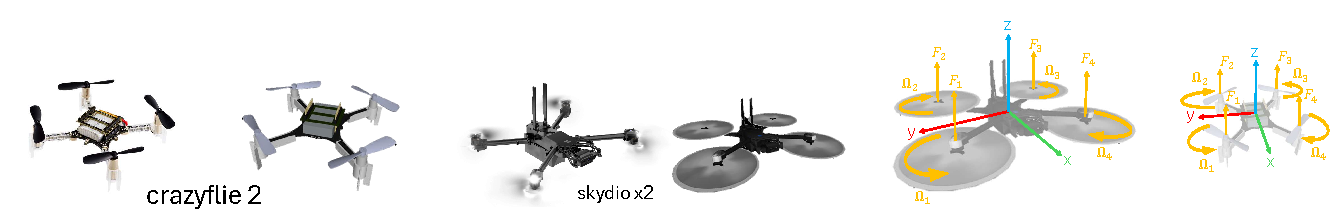
\includegraphics[width=\textwidth]{figures/01_mujoco_missions/fig2_drones_only.pdf}

\caption{Vehicles and simulation models. Left: CF2 hardware and MuJoCo
model. Centre: X2 hardware and MuJoCo model. Right: both geometries at
relative scale. The axis triads are body-frame axes: they are rigidly
attached to the vehicle and therefore rotate with it relative to the
inertial (world) frame (cf.\ $Q\!:\,\text{body}\to\text{inertial}$ in
Sec.~\ref{sec:problem}).}
\label{fig:models}
\end{figure*}


%%%%%%%%%%%%%%%%%%%%%%%%%%%%%%%%%%%%%%%%%%%%%%%%%%%%%%%%%%%%%%%%%%%%%%%%%%
% [v6] Nomenclature. Every symbol that appears in an equation is listed
% once here; the bracketed tag is the equation that defines it.

\begin{comment}
\begin{table*}[t]
\caption{Nomenclature. Parenthesised tags give the defining equation;
vectors are bold; $\clip_{[a,b]}$ and $\sat_{\bm\ell}$ act elementwise.}
\label{tab:nomen}\centering\scriptsize
\setlength{\tabcolsep}{4pt}
\renewcommand{\arraystretch}{0.84}
\begin{tabular}{@{}l>{\raggedright\arraybackslash}p{0.185\textwidth}l>{\raggedright\arraybackslash}p{0.185\textwidth}l>{\raggedright\arraybackslash}p{0.185\textwidth}@{}}
\toprule
\multicolumn{6}{@{}l}{\textit{Attitude, plant, and notation}}\\
$q,\;q_d$ & state / reference quaternion & $q_e$ & error quaternion, $q_d\otimes q^{-1}$ & $q_{e,0},\bm q_{e,v}$ & scalar and vector parts\\
$\bm e_q$ & shortest-path error \eqref{eq:theta} & $\theta_q$ & error angle \eqref{eq:theta} & $\bm\omega$ & body angular rate\\
$J$ & inertia tensor & $Q$ & body-to-inertial rotation & $\otimes$ & quaternion product\\
$\bm\omega_d,\bm\omega_e$ & reference and error rate \eqref{eq:errkin} & $R(\cdot)$ & rotation matrix of a quaternion & $z,z_d,\dot z$ & height, reference, rate \eqref{eq:collective}\\
$\odot,\oslash$ & elementwise $\times$, $\div$ & $\sgnp$ & sign, with $\sgnp(0)=1$ & $\sigma$ & logistic function\\
$I_m$ & identity of order $m$ & $\R$ & real numbers & $\Pi$ & Euclidean projection\\
\midrule
\multicolumn{6}{@{}l}{\textit{Fixed baseline and actuator interface}}\\
$\bm\tau_0=\bm u_0$ & baseline torque \eqref{eq:pd} & $K_q,K_\omega$ & PD gains \eqref{eq:pd} & $\bm\tau_{\max}$ & per-axis torque bound\\
$\omega_n,\zeta$ & design frequency, damping & $\bm\ell$ & per-channel command bound & $\sat_{\bm\ell}$ & saturation at $\pm\bm\ell$\\
$B$ & allocation matrix \eqref{eq:allocationmatrix} & $\bm f$ & rotor forces \eqref{eq:mixer} & $T$ & collective thrust \eqref{eq:collective}\\
$\kappa_i$ & rotor reaction coefficient & $m$ & torque channels, $m=3$ & $M$ & vehicle mass\\
$\bm f_{\max}$ & per-rotor force bound & $g$ & gravity, $9.81$\,m/s$^2$ & $\bm 1$ & vector of ones\\
\midrule
\multicolumn{6}{@{}l}{\textit{Coupled membrane--gate unit}}\\
$v_j$ & membrane state \eqref{eq:cmg} & $r_j$ & gate state \eqref{eq:cmg} & $c_j$ & shunt conductance \eqref{eq:cmg}\\
$\bar{\bm u}$ & normalized baseline \eqref{eq:encoding} & $\bm I^{\pm},\bm I$ & paired currents \eqref{eq:encoding} & $I_b,I_g$ & current offset and gain\\
$\tau,\tau_r$ & membrane, gate time constants & $v_{\rm th}$ & gate threshold & $v_{\rm rest},v_{\rm reset}$ & rest level, reversal level\\
$\gamma$ & gate self-coupling & $\alpha_h$ & logistic sharpness & $\chi$ & conductance switch, $\chi\in\{0,1\}$\\
$g_0,g_1$ & conductance gains (distinct from $g$) & $G$ & activity gain, $G=10^5$ & $h$ & integration step\\
$b_{j,k}$ & gate target \eqref{eq:gate_step} & $r^+_{j,k},v^+_{j,k}$ & updated states \eqref{eq:mem_step} & $\lambda_{j,k},d_{j,k}$ & frozen membrane coefficients\\
\midrule
\multicolumn{6}{@{}l}{\textit{Decoder, online learning, and residual authority}}\\
$\bm a_k$ & clipped activity \eqref{eq:readout} & $W_k$ & decoder \eqref{eq:readout} & $W_0$ & initial decoder, $[I_m,-I_m]$\\
$\bm s_k$ & clipped readout \eqref{eq:readout} & $\bm y^*_k$ & PES target \eqref{eq:pes} & $\bm\varepsilon_k$ & PES error \eqref{eq:pes}\\
$k_e,k^*_\omega$ & target gains \eqref{eq:pes} & $\eta$ & per-step learning rate & $\lambda_W$ & per-step decoder decay\\
$\Pi_{\mathcal W},W_{\max}$ & projection and weight bound & $\beta$ & residual authority \eqref{eq:residual} & $\bm u_k,\bm\delta_k$ & applied command, deviation \eqref{eq:residual}\\
\midrule
\multicolumn{6}{@{}l}{\textit{Reported metrics}}\\
$\bar\theta_q$ & mean quaternion-angle error & $S$ & actuator-bound occupancy [\%] & $n$ & runs per reported cell\\
\bottomrule
\end{tabular}
\end{table*}
\end{comment}

\section{Attitude Baseline and Actuator Interface}
\label{sec:problem}
%%%%%%%%%%%%%%%%%%%%%%%%%%%%%%%%%%%%%%%%%%%%%%%%%%%%%%%%%%%%%%%%%%%%%%%%

The objective is to reduce shortest-path attitude error for a prescribed
$q_d(t)$ while respecting rotor-force limits. Baseline and augmented
controllers share the state measurements, height loop, and allocator;
Section~\ref{sec:architecture} modifies only the requested attitude torque.

%\input{figure1_interface.tex}

\subsection{Quaternion Convention and Error}
Let $Q\in\mathbb S^3$ denote the scalar-first Hamilton quaternion representing attitude (body to inertial), and let $\bm\omega$ be the body angular velocity. For a rigid body with inertia $\bm J\succ0$ about the center of mass, expressed in body axes (cf.~Fig.~\ref{fig:models}), the free-flight rotational dynamics are \cite{schaub2018amss}
\begin{align}
 \dot Q&=\tfrac12 Q\otimes[0,\bm\omega\T]\T,\\
 \bm J\dot{\bm\omega}&=\bm\tau_{\rm act}+\bm\tau_{\rm p}
       +\bm\tau_{\rm d}-\bm\omega\times(\bm J\bm\omega).
 \label{eq:plant}
\end{align}
Here $\bm\tau_{\rm p}$ denotes modeled passive torque and $\bm\tau_{\rm d}$ any applied disturbance; the nominal ideal rigid-body model sets both to zero. Contact, if present, contributes an additional external wrench.

We work with the corresponding passive quaternion $q=Q^{-1}$ \cite{diebel2006quaternion}, which satisfies
\begin{equation}
 \dot q=-\tfrac12[0,\bm\omega\T]\T\otimes q.
 \label{eq:passive}
\end{equation}
The desired attitude $q_d$ uses the same convention. Define the attitude error
\begin{align}
 q_e&=q_d\otimes q^{-1}=[q_{e,0},\bm q_{e,v}\T]\T,\\
 \bm e_q&=\sgnp(q_{e,0})\bm q_{e,v},\qquad \sgnp(0)=1,\\
 \theta_q&=2\operatorname{atan2}(\|\bm q_{e,v}\|_2,|q_{e,0}|)
             \in[0,\pi].
 \label{eq:theta}
\end{align}
The reported error $\theta_q$ is the shortest rotation angle, invariant under $q_e\mapsto-q_e$. Sign selection introduces a discontinuity at $q_{e,0}=0$; it does not establish robust hybrid global stability \cite{mayhew2011hybrid}.

For a desired-frame rate $\bm\omega_d$ satisfying the corresponding passive kinematics, differentiation gives
\begin{align}
 \dot q_e&=\tfrac12q_e\otimes[0,\bm\omega_e\T]\T,\\
 \bm\omega_e&=\bm\omega-R(q_e)\T\bm\omega_d,\qquad
 \dot q_{e,0}=-\tfrac12\bm q_{e,v}\T\bm\omega_e.
 \label{eq:errkin}
\end{align}
These are kinematic identities (no convergence implied). Reference Euler triples parameterize $q_d$ in this passive convention.

\subsection{Physical Inertia and Implemented PD Gains}
Let $\bm J\succ0$ denote the rigid-body inertia about the center of mass, expressed in body axes \cite{schaub2018amss}. When principal moments $\bm j_{\rm p}$ are specified in a rotated principal-axis frame, the physical body-frame tensor is
\begin{equation}
 \bm J=R_{BI}\operatorname{diag}(\bm j_{\rm p})R_{BI}\T,
 \label{eq:inertiaframe}
\end{equation}
for the rotation from principal axes to body axes $R_{BI}$. The implementation sets axiswise gains using the principal moments in their reported ordering, $\bm j_{\rm tune}$, not necessarily $\operatorname{diag}(\bm J)$ (Table~\ref{tab:models}).

The fixed quaternion PD baseline is
\begin{align}
 \bm k_q&=2\bm j_{\rm tune}\odot\bm\omega_n^2,\qquad
 \bm k_\omega=2\zeta\bm j_{\rm tune}\odot\bm\omega_n,\\
 \bm u_0&=\sat_{\bm\ell}
       (-\bm k_q\odot\bm e_q-\bm k_\omega\odot\bm\omega),
 \label{eq:pd}
\end{align}
where $\odot$ denotes componentwise multiplication,
$\bm\omega_n=(4,4,3.5)\T$ rad/s, $\zeta=0.95$, and
$\sat_{\bm\ell}$ clips component $i$ to $[-\ell_i,\ell_i]$.
%
The requested-torque box is $\mathcal U=\prod_{i=1}^3[-\ell_i,\ell_i]$;
$\clip_{[a,b]}$ also acts componentwise, and $\oslash$ denotes componentwise division.
We impose componentwise torque limits $\bm\ell\in\mathbb R_{>0}^3$ through $\sat_{\bm\ell}(\cdot)$. In our implementation, $\bm\ell$ is chosen proportional to the diagonal gain-scheduling vector $\bm j_{\rm tune}$ via
$\ell_i=\max(j_{{\rm tune},i}\nu_i,10^{-6}\ \mathrm{N\,m})$,
with acceleration-scale vector $\bm\nu=(12,12,10)\T$ rad/s$^2$.
These controller-side bounds are not the rotor-feasible torque set.
%
The law is quaternion feedback \cite{fresk2013quaternion}; $\bm\omega_n$ is a tuning parameter rather than a claimed set of coupled closed-loop natural frequencies.
Desired-rate feedforward and gyroscopic cancellation are omitted.
The resulting gains are vehicle-specific through $\bm j_{\rm tune}$, even though
$\bm\omega_n$ and $\zeta$ are shared; the same fixed gains are then retained
for PD and its CMG augmentation.
The local result in Section~\ref{sec:local} uses these anisotropic gains; it does not replace them with a scalar-gain controller.
%
\subsection{Requested and Realized Wrench}
For rotor positions $\bm p_i$ in body coordinates, parallel $+z$ thrust
axes, and signed reaction coefficients $\kappa_i$, define
\begin{equation}
 B=\begin{bmatrix}
 1&1&1&1\\p_{1,y}&p_{2,y}&p_{3,y}&p_{4,y}\\
 -p_{1,x}&-p_{2,x}&-p_{3,x}&-p_{4,x}\\
 \kappa_1&\kappa_2&\kappa_3&\kappa_4
 \end{bmatrix}.
 \label{eq:allocationmatrix}
\end{equation}
The signs follow $\bm p_i\times[0,0,f_i]\T$ and the actuator's local reaction torque $\kappa_i f_i$. Here $B$ maps rotor thrusts to total thrust and body torque; $\kappa_i$ has units of meters, not angular velocity. Given a commanded collective thrust $T$ and body-torque command $\bm u$, the corresponding inverse-allocation and clipping model is
\begin{equation}
 \begin{aligned}
 \bm f_{\rm req}&=B^{-1}[T,\bm u\T]\T,\\
 \bm f_{\rm act}&=\clip_{[\bm0,\bm f_{\max}]}(\bm f_{\rm req}),\\
 [T_{\rm act},\bm\tau_{\rm act}\T]\T&=B\bm f_{\rm act}.
 \end{aligned}
 \label{eq:mixer}
\end{equation}
Here $\bm u=\bm u_0$ for PD; the CMG path in Section~\ref{sec:architecture}
modifies that requested torque before the same allocation and clipping.
Each $f_i$ is a commanded force in newtons, not a rotor-speed command.
Exact wrench realization requires
$B^{-1}[T,\bm u\T]\T\in[\bm0,\bm f_{\max}]$.
A componentwise torque box is not generally contained in this
collective-dependent feasible set. Clipped inverse allocation is used,
not an optimization-based allocator \cite{monteiro2016allocation}.

Collective thrust remains classical, with $z_d=1$ m:
\begin{equation}
 T=\clip_{[0,2.5Mg]}
 \left(\frac{M[g+6(z_d-z)-4\dot z]}{\max(R(Q)_{33},0.35)}\right).
 \label{eq:collective}
\end{equation}
Here $g$ is the gravitational acceleration. The height loop reads altitude and vertical velocity; the denominator compensates tilt.
The guard $0.35$ prevents near-singular tilt compensation as $R(Q)_{33}\to0$
(i.e., near $90^\circ$ tilt) and corresponds to limiting the effective
compensation to about $\arccos(0.35)\approx69.5^\circ$. Its upper bound does
not supersede individual rotor limits. The CMG path has no direct collective
output, but can affect height through attitude, tilt compensation, and
allocation saturation.
The resulting shared plant interface isolates changes in requested
attitude torque while preserving the same physical simulation for both
controllers.

%%%%%%%%%%%%%%%%%%%%%%%%%%%%%%%%%%%%%%%%%%%%%%%%%%%%%%%%%%%%%%%%%
\section{CMG State Dynamics and Online Decoder Adaptation}
\label{sec:architecture}
\label{sec:analysis}
%%%%%%%%%%%%%%%%%%%%%%%%%%%%%%%%%%%%%%%%%%%%%%%%%%%%%%%%%%%%%%%%%
This section specifies the residual architecture in state-space form and the online decoder update, then states the boundedness properties that follow from the resulting saturations and projections.
\subsection{Encoding, States, and Numerical Update}

For $m$ torque channels and $2m$ units, normalize the clipped baseline and
form positive/negative current pairs:
\begin{equation}
 \begin{aligned}
 \bar{\bm u}&=\bm u_0\oslash\bm\ell,\\
 \bm I^{\pm}&=I_b\bm1+I_g\max(\pm\bar{\bm u},\bm0),\\
 \bm I&=[(\bm I^+)\T,(\bm I^-)\T]\T.
 \end{aligned}
 \label{eq:encoding}
\end{equation}
Each unit has a dimensionless membrane state $v_j$ and gate $r_j$:
\begin{align}
 \dot r_j&=[\sigma(\alpha_h(v_j-v_{\rm th}+\gamma r_j))-r_j]/\tau_r,\\
 \dot v_j&=-(v_j-v_{\rm rest})/\tau+I_j/\tau-c_j(v_j-v_{\rm reset}),\\
 c_j&=(g_0+\chi g_1|I_j|)r_j^2,\qquad \chi\in\{0,1\}.
 \label{eq:cmg}
\end{align}
% [v6] CMG unit coupling topology (TikZ source under architectures/tikz/).
\begin{figure}[t]
\centering
\resizebox{0.86\columnwidth}{!}{% B1c -- column-native CMG unit: coupling topology only. The state
% equations stay in the text; the figure shows which variable acts on which.
% Natural width is about one IEEE column, so no \resizebox is needed.
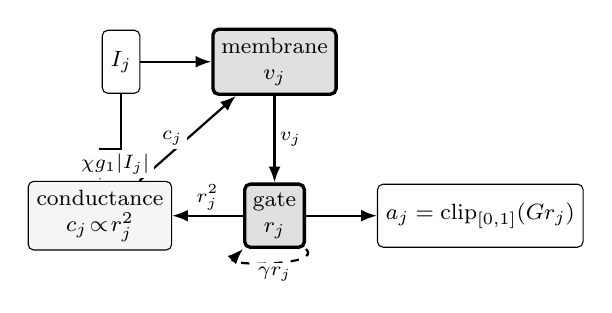
\begin{tikzpicture}[node distance=6mm and 9mm,font=\footnotesize]
  \node[blk]                       (I) {$I_j$};
  \node[neuro,right=of I]          (v) {membrane\\$v_j$};
  \node[neuro,below=11mm of v]     (r) {gate\\$r_j$};
  \node[clas,left=of r]            (c) {conductance\\$c_j\!\propto\! r_j^{2}$};
  \node[blk,right=of r]            (a) {$a_j=\clip_{[0,1]}(G r_j)$};

  \draw[sig] (I) -- (v);
  \draw[sig] (v.south) -- node[lbl,right]{$v_j$} (r.north);
  \draw[sig] (r) -- node[lbl,above]{$r_j^{2}$} (c);
  \draw[sig] (c) -- node[lbl,left]{$c_j$} (v);
  \draw[sig] (r) -- (a);
  \draw[sigd] (r.south east) to[out=-45,in=-135]
        node[lbl,below]{$\gamma r_j$} (r.south west);
  \draw[sig] (I.south) -- ++(0,-7mm) -| node[lbl,pos=.14,below]{$\chi g_1|I_j|$} (c.north);
\end{tikzpicture}
}
\caption{Coupling topology of one CMG unit, cf.~\eqref{eq:cmg}. The
membrane sets the gate target; the gate acts back twice, shifting its own
threshold through $\gamma$ and shunting the membrane through
$c_j\propto r_j^2$ ($\chi=1$ makes that shunt input dependent). The
dynamics are continuous: no spike, no reset, and only $a_j$ leaves the
unit.}
\label{fig:cmgunit}
\end{figure}
%
The logistic gate target depends on $v_j$, while $r_j$ shifts that target
and modulates membrane conductance (Fig.~\ref{fig:cmgunit}). Thus, both states participate even
though the decoder reads the gate-derived activity. The model has no
threshold-triggered reset or spike event; $v_{\rm reset}$ is a reversal
level in a continuous conductance term. The gains $g_0,g_1$ have the units
needed to make $c_j$ a rate.

The actual integration is sequential, not exponential Euler for both
states. From the old states compute
\begin{align}
 b_{j,k}&=\sigma\!\left(\clip_{[-60,60]}
       [\alpha_h(v_{j,k}-v_{\rm th}+\gamma r_{j,k})]\right),\\
 r_{j,k}^{+}&=\clip_{[0,1]}
       [r_{j,k}+(h/\tau_r)(b_{j,k}-r_{j,k})].
 \label{eq:gate_step}
\end{align}
Then evaluate $c_{j,k}=(g_0+\chi g_1|I_{j,k}|)(r_{j,k}^{+})^2$,
$\lambda_{j,k}=\tau^{-1}+c_{j,k}$, and
$d_{j,k}=(v_{\rm rest}+I_{j,k})/\tau+c_{j,k}v_{\rm reset}$. The
frozen-coefficient membrane step is
\begin{equation}
 v_{j,k}^{+}=e^{-\lambda_{j,k}h}v_{j,k}
       +(1-e^{-\lambda_{j,k}h})d_{j,k}/\lambda_{j,k}.
 \label{eq:mem_step}
\end{equation}
This exactly solves the scalar membrane equation with those frozen
coefficients; it does not establish unconditional stability of the coupled
nonlinear closed loop. Assign $(v_{j,k+1},r_{j,k+1})=(v_{j,k}^{+},r_{j,k}^{+})$.

\subsection{Readout, PES, and Additive Residual}
The within-step activity, initial decoder, and clipped readout are
\begin{equation}
 \begin{aligned}
 \bm a_k&=\clip_{[0,1]}(G\bm r_k^+),\qquad W_0=[I_m,-I_m],\\
 \bm s_k&=\clip_{[-1,1]}(W_k\bm a_k).
 \end{aligned}
 \label{eq:readout}
\end{equation}
Pair subtraction retains directional information from a nonnegative
activity basis; state memory does not imply instantaneous sign agreement
after a command reversal. With $G=10^5$ the activity saturates once
$r_j\ge10^{-5}$, so $G$ is a primary design hyperparameter for how much of
$r_j$'s dynamic range reaches the decoder. The teaching target and local update are
\begin{align}
 \bm y_k^*&=\clip_{[-1,1]}(-k_e\bm e_{q,k}-k_\omega^*\bm\omega_k),\\
 \bm\varepsilon_k&=\bm y_k^*-\bm s_k,\\
 W_{k+1}&=\Pi_{\mathcal W}
       [W_k+\eta\bm\varepsilon_k\bm a_k\T-\lambda_W W_k].
 \label{eq:pes}
\end{align}
Here $\mathcal W=[-W_{\max},W_{\max}]^{m\times2m}$. The coefficients $\eta$ and $\lambda_W$ are per-step (so changing $h$ changes the effective learning dynamics). PES is a local error-driven update toward the prescribed target $\bm y_k^*$; it does not differentiate through the plant or claim to minimize a closed-loop cost.

Using $W_k$ before the update, the requested command is
\begin{equation}
 \bm u_k=\sat_{\bm\ell}(\bm u_{0,k}+\beta\bm\ell\odot\bm s_k),\quad
 \bm\delta_k=\bm u_k-\bm u_{0,k},\quad 0\le\beta\le1.
 \label{eq:residual}
\end{equation}
The canonical UAV case has $m=3$, six CMG units, and eighteen decoder
weights. Intrinsic conductance modulation ($\chi$), synaptic/decoder
adaptation ($W_k$), and output authority ($\beta\bm\ell$) are distinct.

\subsection{Structural Properties and Their Scope}
We first state the boundedness properties that follow directly from the architecture: internal-state bounds, a uniform command-deviation bound set by residual authority, and projection-based bounds on decoder weights.
\begin{proposition}[Bounded internal states]
With the nonnegative conductance parameters in Table~\ref{tab:parameters},
$r_{j,0}\in[0,1]$, and $0<h\le\tau_r$, the gate remains in $[0,1]$.
The membrane iterate remains in the convex hull of its initial value,
$v_{\rm reset}$, and the interval
$[v_{\rm rest}+I_b,v_{\rm rest}+I_b+I_g]$.
\end{proposition}
\begin{proof}
The unclipped gate step is a convex combination of $r_{j,k}$ and
$b_{j,k}\in[0,1]$. Since $I_j\in[I_b,I_b+I_g]$ and $c_j\ge0$,
$d_j/\lambda_j$ is a convex combination of $v_{\rm rest}+I_j$ and
$v_{\rm reset}$. Equation~\eqref{eq:mem_step} is a convex combination of
$v_{j,k}$ and $d_j/\lambda_j$. Induction proves both statements.
\end{proof}

\begin{proposition}[Bounded authority and baseline recovery]
\label{prop:authority}
For $\bm u_{0,k}\in\mathcal U$ and any finite $W_k$,
$\bm u_k\in\mathcal U$ and $|\delta_{k,i}|\le\beta\ell_i$.
If $\beta=0$, the requested baseline command is recovered at every step.
If $W_k=0$ at a particular step, it is recovered at that step, but learning
need not keep $W_{k+1}=0$.
\end{proposition}
\begin{proof}
The outer clip enforces membership in $\mathcal U$. Its componentwise
nonexpansiveness and $\sat_{\ell_i}(u_{0,k,i})=u_{0,k,i}$ give
$|\delta_{k,i}|\le|\beta\ell_i s_{k,i}|\le\beta\ell_i$.
The recovery statements follow by substitution.
\end{proof}
The same allocator and state then give the same actuator output when
$\beta=0$. The proposition does not establish state safety, rotor
headroom, stability, or a bound on tracking improvement. A bounded
adversarial correction can still degrade or destabilize a nonlinear plant.

\begin{proposition}[Decoder bound and restricted contraction]
\label{prop:pes}
If $W_0\in\mathcal W$, then \eqref{eq:pes} keeps $W_k\in\mathcal W$.
If, additionally, the target and a nonzero activity $\bm a$ are fixed,
leak is zero, and readout clipping and projection remain inactive, then
\begin{equation}
 \bm\varepsilon_{k+1}
       =(1-\eta\|\bm a\|_2^2)\bm\varepsilon_k.
 \label{eq:contraction}
\end{equation}
For a nonzero initial error, its norm contracts to zero when
$0<\eta\|\bm a\|_2^2<2$.
\end{proposition}
\begin{proof}
Projection gives the first result. Under the additional conditions,
$(W_{k+1}-W_k)\bm a=\eta\bm\varepsilon_k\|\bm a\|_2^2$;
subtracting this from the fixed target error gives
\eqref{eq:contraction}. The scalar multiplier has modulus less than one
under the stated condition.
\end{proof}
This is the constant-feature PES result \cite{voelker2015pes}, not a
closed-loop convergence theorem. Since $\|\bm a\|^2\le2m$,
$0<\eta<1/m$ is sufficient for that restricted model with nonzero
activity; changing targets, loss of excitation, clipping, and leakage
invalidate a direct application to the experiment. No unique identification
of all decoder weights follows from one fixed regressor.

% [v7] The statement a control audience looks for first. Scoped: it is a
% conditional bound, not a stability theorem, and says so.
%\begin{remark}[Scope of a small-gain argument]
%\label{rem:smallgain}
%Propositions~\ref{prop:authority} and \ref{prop:pes} place the realized
%command deviation in a known box, $|\delta_{k,i}|\le\beta\ell_i$, uniformly
%in $k$ and independently of what the decoder has learned. If the baseline
%loop is input-to-state stable with respect to an additive torque
%perturbation, with gain $\gamma(\cdot)$ on that input, then the augmented
%loop inherits an ISS estimate with asymptotic bound
%$\gamma(\beta\|\bm\ell\|)$, and $\beta$ tunes it continuously to zero. Two
%conditions are not discharged here. The perturbation entering the plant is
%post-allocation, so the relevant bound is on $B^{-1}$ applied to
%$\bm\delta_k$ under rotor saturation, not on $\bm\delta_k$ itself; and the
%required ISS gain for the saturated quaternion-PD baseline is not
%established in this paper. The architecture therefore supplies the bounded
%perturbation such an argument needs, and identifies the two missing
%ingredients, without asserting the conclusion.
%\end{remark}

\subsection{Allocation-Aware Local Stability}
\label{sec:local}
Let $E=[\bm0_{3\times1},I_3]\T$, $H=E\T$, and let
$\mathcal A_T(\bm u)=HB\clip_{[0,\bm f_{\max}]}(B^{-1}[T,\bm u\T]\T)$
be the realized torque at collective $T$. For two commands at the
\emph{same state and collective}, scalar clipping has secant slopes
$d_i\in[0,1]$. Consequently,
\begin{align}
 \mathcal A_T(\bm u)-\mathcal A_T(\bm u_0)
 &=HBDB^{-1}E\bm\delta,\\
 \|\mathcal A_T(\bm u)-\mathcal A_T(\bm u_0)\|_2
 &\le L_A\beta\|\bm\ell\|_2,
 \label{eq:allocbound}
\end{align}
where $D=\operatorname{diag}(d_i)$ and
$L_A=\max_{D\in\mathcal D}\|HBDB^{-1}E\|_2$.
$\mathcal D$ is the set of sixteen diagonal matrices with entries
in $\{0,1\}$. The vertex maximum bounds all intermediate $D$ by convexity.
This holds even with rotor clipping, but is not a bound between two
different closed-loop trajectories. It also does not bound the height error.

For a constant reference and a smooth shortest-path branch, let
$\bm x=[\bm e_q\T,\bm\omega\T]\T$ and
$K_q=\operatorname{diag}(\bm k_q)$, $K_\omega=\operatorname{diag}(\bm k_\omega)$.
Write the continuous-time attitude subsystem as
\begin{equation}
 \begin{gathered}
 \dot{\bm x}=A\bm x+\bm g(\bm x)+F\bm d,\\
 A=\begin{bmatrix}0&\frac12I_3\\-\bm J^{-1}K_q&-\bm J^{-1}K_\omega\end{bmatrix},
 \qquad F=\begin{bmatrix}0\\\bm J^{-1}\end{bmatrix},
 \end{gathered}
 \label{eq:localmodel}
\end{equation}
where $\bm d=\bm\tau_{\rm act}+\bm\tau_{\rm p}+\bm\tau_{\rm d}
 +K_q\bm e_q+K_\omega\bm\omega$ is the total deviation from ideal PD torque.
It includes allocation and command-saturation errors, not just the neural
request. The nonlinear remainder is
\begin{equation}
 \bm g(\bm x)=\begin{bmatrix}
 \tfrac12[(\sqrt{1-\|\bm e_q\|^2}-1)I_3+[\bm e_q]_\times]\bm\omega\\
 -\bm J^{-1}[\bm\omega]_\times\bm J\bm\omega
 \end{bmatrix}=O(\|\bm x\|^2),
 \label{eq:localremainder}
\end{equation}
with $[\bm z]_\times\bm y=\bm z\times\bm y$. Norms below use fixed
coordinates with angular rates expressed in rad/s.

\begin{theorem}[Conditional local practical stability]
\label{thm:local}
Let $\bm J,K_q,K_\omega\succ0$, let $q_d$ be constant, and use the smooth
branch in \eqref{eq:localmodel}. Choose $Q_L\succ0$ and the solution
$P\succ0$ of $A\T P+PA=-Q_L$. On $\|\bm x\|\le r<1$, suppose
$\|\bm g(\bm x)\|\le L_r\|\bm x\|^2$ and choose $r$ so that
$c=\lambda_{\min}(Q_L)-2\|P\|L_r r>0$.
Set $p_- =\lambda_{\min}(P)$, $p_+=\lambda_{\max}(P)$,
$b=\|PF\|$, and $V=\bm x\T P\bm x$. If
\begin{equation}
 V(0)\le p_-r^2,\qquad
 \|\bm d(t)\|\le\bar d<\frac{cr}{2b}\sqrt{\frac{p_-}{p_+}},
 \label{eq:localsmallness}
\end{equation}
then $V\le p_-r^2$ is forward invariant and
\begin{equation}
 V(t)\le e^{-\alpha t}V(0)+\frac{4p_+b^2}{c^2}\bar d^2,
 \qquad \alpha=\frac{c}{2p_+}.
 \label{eq:localiss}
\end{equation}
Thus attitude regulation is locally input-to-state stable; zero
perturbation gives local exponential convergence of the plant state.
\end{theorem}
\begin{proof}
The linear system has energy
$\frac12\bm\omega\T\bm J\bm\omega+\bm e_q\T K_q\bm e_q$ with derivative
$-\bm\omega\T K_\omega\bm\omega$. Its only invariant zero-derivative
trajectory is the origin, so $A$ is Hurwitz and $P\succ0$ exists.
Equations~\eqref{eq:localmodel}--\eqref{eq:localremainder} give
\[
 \dot V\le-c\|\bm x\|^2+2b\|\bm x\|\bar d
 \le-\frac c2\|\bm x\|^2+\frac{2b^2}{c}\bar d^2.
\]
On $V=p_-r^2$, $\|\bm x\|\ge r\sqrt{p_-/p_+}$, so
\eqref{eq:localsmallness} makes the first bound strictly negative.
The ellipsoid stays inside the radius-$r$ ball; integration of
$\dot V\le-\alpha V+2b^2\bar d^2/c$ gives \eqref{eq:localiss}.
\end{proof}

If the same-state baseline deviation from ideal PD is bounded by $\bar d_0$,
then \eqref{eq:allocbound} permits
$\bar d=\bar d_0+L_A\beta\|\bm\ell\|$ in the theorem, \emph{provided}
\eqref{eq:localsmallness} holds. This is a sufficient local robustness
condition, independent of the particular PES trajectory, not a PES
convergence proof. Numerical checks confirm that $A$ is Hurwitz for both
implemented gain sets. The smallness condition has not been certified
for the experimental $\beta=0.5$. Moving references, the $180^\circ$
sign boundary, sampled-data/solver error, and full translational stability
remain outside this result; sample-and-hold error would need its own
bound within $\bm d$.

\paragraph{Nengo realization.}
In Nengo~4.1.0, a custom \texttt{NeuronType} exposes membrane and gate states. Direct current injection into \texttt{ensemble.neurons} bypasses NEF gain/intercept fitting. Unfiltered CMG activity uses $\eta_N=\eta(2m)/h$ and Nengo error $\bm s-\bm y^*$. Leak uses pre-step weights; projection follows the simulator step. Nengo's teaching graph introduces a one-step latency, so this is not an identical weight sequence. The maximum relative mean-error difference over ten direct/Nengo cases is $2.013\times10^{-6}$, a tested numerical agreement rather than formal backend equivalence.


\section{Experimental Protocol and Cross-Mission Results}
\label{sec:results}
\subsection{Models, Parameters, and Measurements}

MuJoCo provides rigid-body simulation with site-applied actuator wrenches \cite{todorov2012mujoco}. We evaluate two Menagerie-derived multirotor models \cite{menagerieModels} (CF2 and X2) as free-flying rigid bodies: the attitude loop commands three body torques and a separate height loop commands collective thrust.

The upstream CF2 model exposes abstract moment channels \cite{menagerieCF2}; we replace them with four rotor-force channels and the shared clipped inverse allocator \eqref{eq:mixer} to expose thrust/torque coupling and per-rotor limits. Rotor ordering is $(-x,-y),(-x,+y),(+x,+y),(+x,-y)$ with reaction signs $(-,+,-,+)$. Table~\ref{tab:models} separates simulation/interface parameters from manufacturer context; the CF2 $1.5\times$ scale increases a model limit, not measured hardware capability. Both models are simplified (no motor/RPM/battery states and no validated rotor aerodynamics); feedback uses \texttt{qpos}/\texttt{qvel}, with noise injected only in Sec.~\ref{sec:noise}.

\begin{table}[t]
\centering
\caption{Main model/interface parameters and manufacturer context.
Mass agrees with published CF2/X2 specifications \cite{bitcrazeCF20Specs,skydioX2ESpecs}; force limits, inertias, and reaction coefficients are simulation parameters, not identified hardware ratings.}
\label{tab:models}
\setlength{\tabcolsep}{3pt}
\footnotesize
\begin{tabular}{@{}p{0.40\linewidth}p{0.27\linewidth}p{0.25\linewidth}@{}}
\toprule
Parameter & CF2 rotor model & X2 model\\
\midrule
Mass $M$ (kg) & $0.027$ & $1.325$\\
Rotor $|p_x|,|p_y|$ (m) & $0.0325,0.0325$ & $0.14,0.18$\\
Reaction magnitude $|\kappa_i|$ (m) & $0.005$ & $0.0201$\\
Rotor force limit (N) & $.0875\to.13125$ & $13$\\
Total force limit (N) & $.350\to.525$ & $52$\\
Main-test thrust/weight & $1.982$ & $4.001$\\
$\bm j_{\rm tune}$ ($10^{-5}$ kg\,m$^2$) & $(2.3951,\allowbreak2.3951,\allowbreak3.2347)$ & ---\\
$\bm j_{\rm tune}$ ($10^{-2}$ kg\,m$^2$) & --- & $(6.0711,\allowbreak3.6468,\allowbreak2.5412)$\\
Rigid-body integrator & RK4 & Euler\\
Experiment timestep (s) & $0.0005$ & $0.0005$\\
Manufacturer thrust data & $.568$ N\textsuperscript{a} & Not published\textsuperscript{b}\\
\bottomrule
\end{tabular}
\par\smallskip
\begin{minipage}{0.97\linewidth}
\scriptsize
\textsuperscript{a}Historical CF2 measurement at 93.75\% PWM using an external power supply \cite{bitcrazeThrustMeasurements}; not a continuous battery-powered rating. The modeled $.525$ N is below that observation.
\textsuperscript{b}Not reported in the reviewed X2 datasheet. Neither model includes motor lag; a historical CF2 motor step took about 180 ms \cite{bitcrazeMotorResponse}, illustrating an omitted hardware effect.
\end{minipage}
\end{table}

\begin{comment}
\begin{table}[t]
\centering
\caption{Simulation-model characteristics. CF2 authority is scaled relative to the upstream model limit.}
\label{tab:models}
\setlength{\tabcolsep}{3pt}
\footnotesize
\begin{tabular}{@{}p{0.40\linewidth}p{0.27\linewidth}p{0.25\linewidth}@{}}
\toprule
Property & CF2 rotor model & X2 model\\
\midrule
Mass $M$ (kg) & $0.027$ & $1.325$\\
Rotor $|p_x|,|p_y|$ (m) & $0.0325,0.0325$ & $0.14,0.18$\\
Reaction magnitude $|\kappa_i|$ (m) & $0.005$ & $0.0201$\\
Unscaled rotor limit (N) & $0.0875$ & $13$\\
Main-test authority scale & $1.5$ & $1$\\
Main-test rotor limit (N) & $0.13125$ & $13$\\
Main-test total limit (N) & $0.525$ & $52$\\
Maximum thrust/weight & $1.321\to1.982$ & $4.001$\\
Rigid-body integrator & RK4 & Euler\\
Experiment timestep (s) & $0.0005$ & $0.0005$\\
Motor activation/RPM states & None & None\\
\bottomrule
\end{tabular}
\end{table}

\begin{table}[t]
\centering
\caption{Simulation parameters vs. manufacturer information (where available).}
\label{tab:manufacturer}
\setlength{\tabcolsep}{3pt}
\footnotesize
\begin{tabular}{@{}>{\raggedright\arraybackslash}p{0.25\linewidth}>{\raggedright\arraybackslash}p{0.30\linewidth}>{\raggedright\arraybackslash}p{0.37\linewidth}@{}}
\toprule
Quantity & Simulation & Manufacturer information\\
\midrule
CF2 mass & $27$ g & $27$ g \cite{bitcrazeCF20Specs}\\
X2 mass & $1325$ g & $1325$ g with battery \cite{skydioX2ESpecs}\\
CF2 total thrust & $0.350\to0.525$ N & $0.568$ N measured at $93.75\%$ PWM\textsuperscript{a} \cite{bitcrazeThrustMeasurements}\\
X2 rotor limit & $13$ N per rotor & Not reported \cite{skydioX2ESpecs}\\
CF2 motor response & No motor dynamics & $\sim180$ ms: $0\to25{,}000$ RPM\textsuperscript{b} \cite{bitcrazeMotorResponse}\\
Inertia tensors & CF2 inherited; X2 geometry-derived & Not reported in product specifications \cite{bitcrazeCF20Specs,skydioX2ESpecs}\\
\bottomrule
\end{tabular}
\par\smallskip
\begin{minipage}{0.97\linewidth}
\scriptsize
\textsuperscript{a}Historical total-thrust measurement with a power-supply test setup, not a guaranteed continuous battery-powered rating.
\textsuperscript{b}One motor's reported full-command response with a charged battery; not an identified first-order time constant.
\end{minipage}
\end{table}
\end{comment}

CF2's body axes are principal axes. For X2, the geometry-derived body tensor is
\[
 \bm J=10^{-2}\begin{bmatrix}3.66517&0&-.21000\\0&2.54117&0\\-.21000&0&6.05280\end{bmatrix}
 \ \mathrm{kg\,m^2}.
\]
It differs from both $\operatorname{diag}(\bm j_{\rm tune})$ and a
manufacturer-identified tensor. Torque limits use $\bm j_{\rm tune}$ as
defined in Section~\ref{sec:problem}.

Each PD/CMG pair uses the same initial state, reference, duration, allocator, model, and timestep. The primary campaign is nominal and deterministic (no injected disturbances or sensor noise), with one run per cell and learning active throughout. We report the mean error $\bar\theta_q$ and relative reduction $100(\bar\theta_{q,\rm PD}-\bar\theta_{q,\rm CMG})/\bar\theta_{q,\rm PD}$; means use all 90{,}000 samples even when plotted traces are decimated.

\begin{table}[h]
\caption{Canonical 3-channel CMG--PES parameters. Neural states/currents
are normalized model variables; learning coefficients are per step.}
\label{tab:parameters}\centering\small
\begin{tabular}{ll}
\toprule
Quantity & Value\\\midrule
$h$, duration & $0.0005$ s, $45$ s\\
$\tau,\tau_r$ & $0.05$ s, $0.005$ s\\
$v_{\rm rest},v_{\rm reset},v_{\rm th}$ & $0,0,1$\\
$v_{j,0},r_{j,0},\chi$ & $0,0,1$\\
$\alpha_h,\gamma,g_0,g_1$ & $50,2,120,30$\\
$I_b,I_g,G$ & $0.75,1.25,10^5$\\
$\beta,\eta,\lambda_W,W_{\max}$ & $0.5,8\times10^{-4},10^{-6},6$\\
$k_e,k_\omega^*$ & $8,0$\\
\bottomrule
\end{tabular}
\end{table}

The five reference triples are generated as follows (radians):
Roll is $(0.25\sin0.7t,0,0)$; Full3 is
$0.5\sin(t+(0,\pi/2,\pi)\T)$, componentwise. Hard45 is
\begin{equation}
 \begin{bmatrix}
 0.55\sin(0.75t)+0.20\sin(2.10t+0.40)\\
 0.45\sin(0.95t+\pi/3)+0.18\sin(1.75t)\\
 0.65\sin(0.55t+\pi)+0.25\sin(1.35t+0.20)
 \end{bmatrix}.
\end{equation}
Hardstep holds zero for one second, then cycles every two seconds through
the rows of
\begin{equation}
 \begin{bmatrix}
 .75&-.45&.55\\-.65&.55&-.70\\.50&.50&.90\\-.80&-.35&.20
 \end{bmatrix}.
\end{equation}
Yaw360 is $(0,0,2\pi(3\xi^2-2\xi^3))$ with $\xi=t/45$.
The nominal Hover equilibrium is also available, but its essentially zero
error does not support a meaningful percentage comparison.

\begin{figure}[t]
\centering
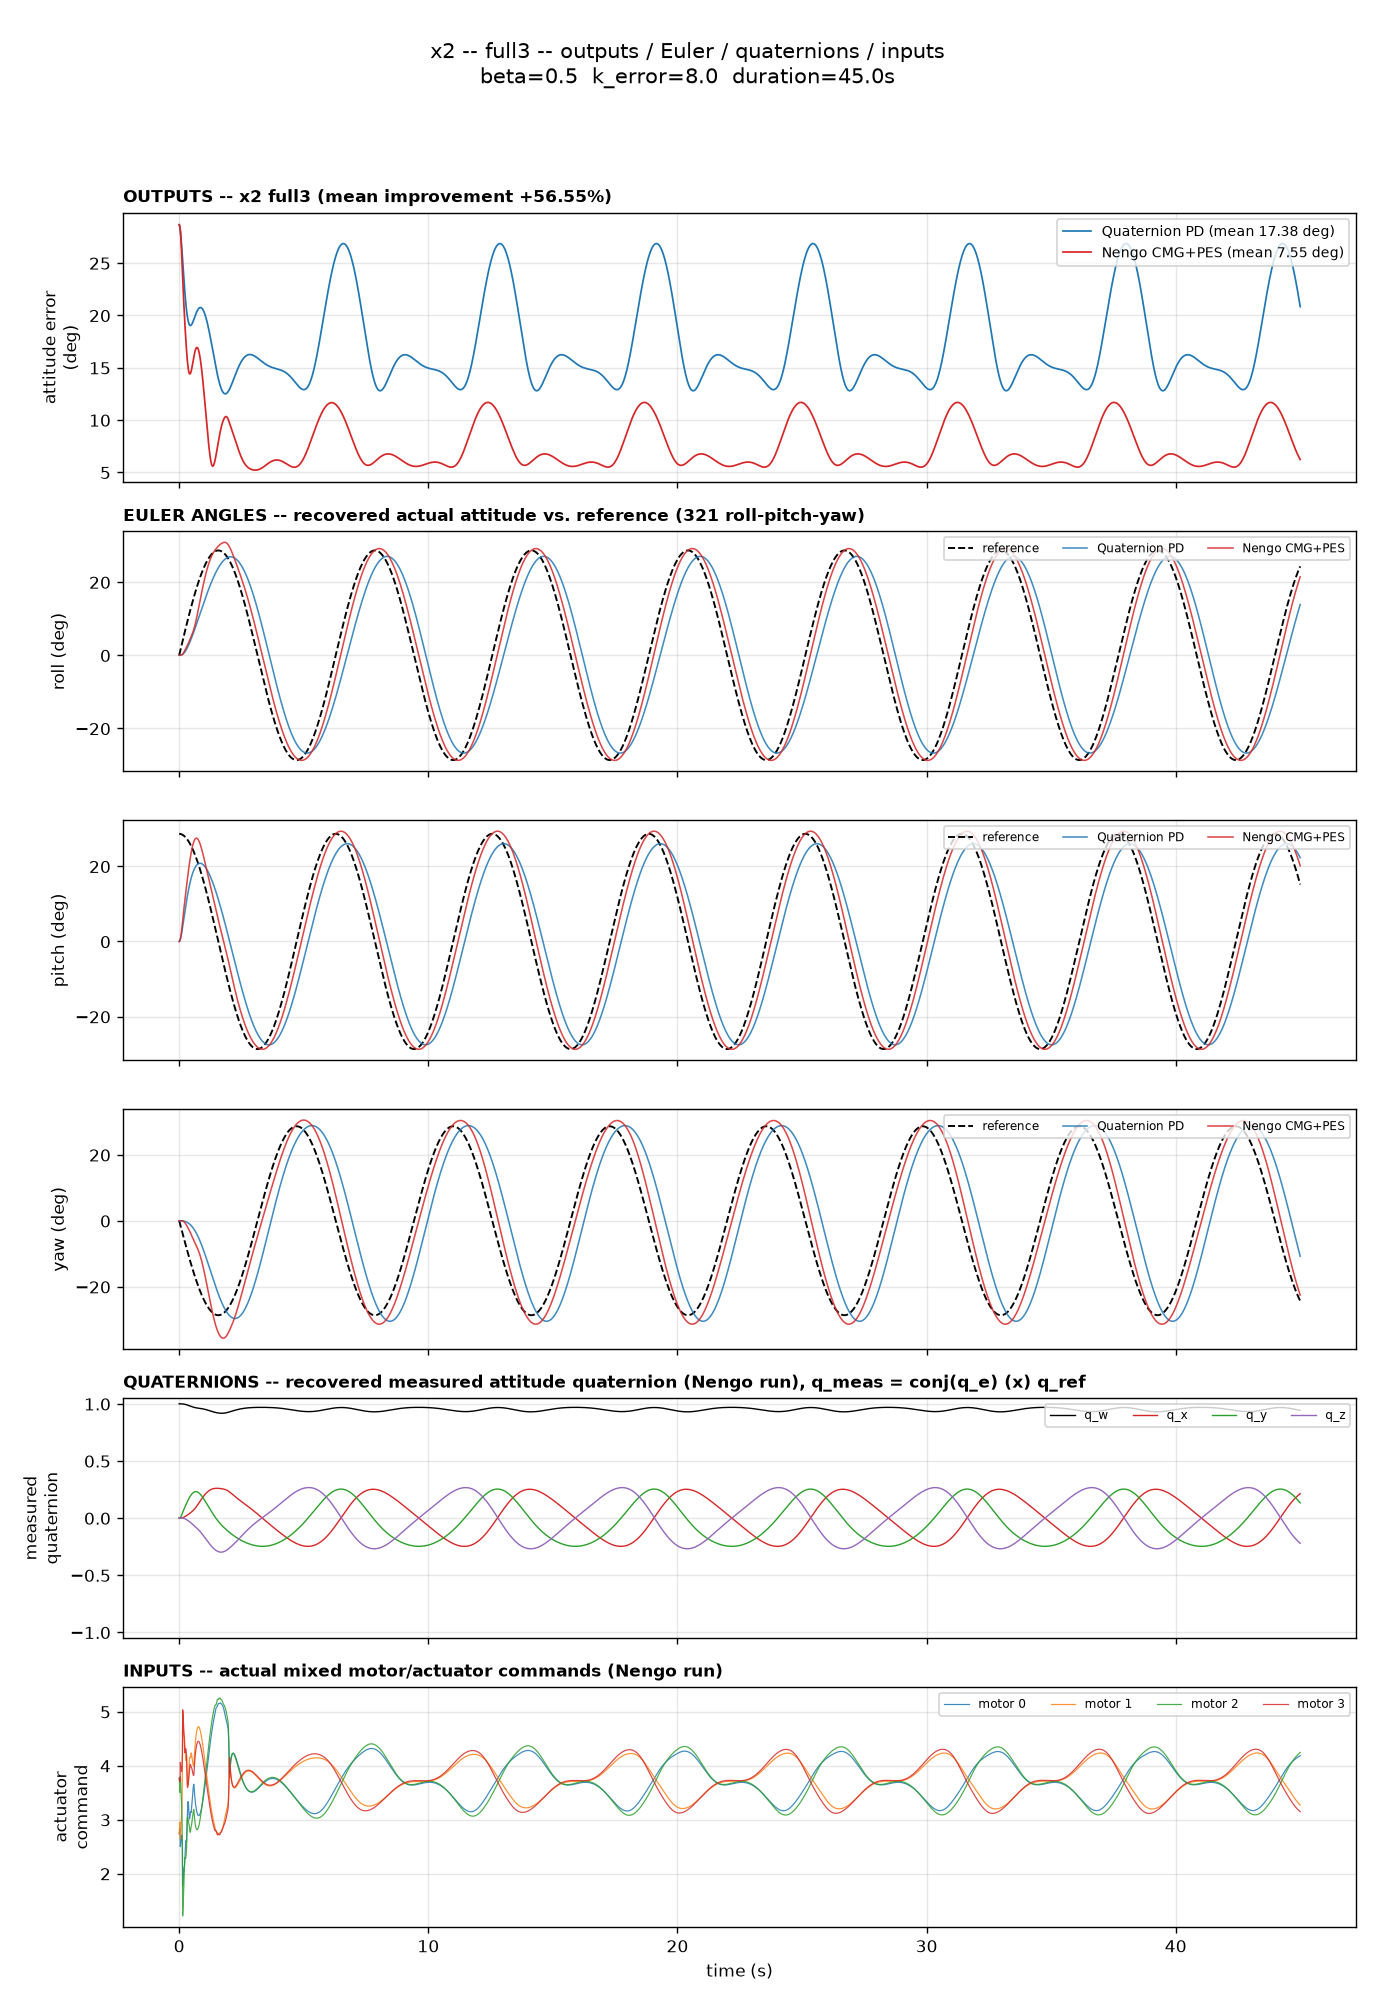
\includegraphics[width=\linewidth]{figures/02_neural_activity/attitude_detail/x2_full3_attitude.png}
\caption{X2 Full3 mission: PD baseline versus CMG--PES augmentation over the
45-s run. Full3 commands all three axes simultaneously and is the largest
reduction that is also insensitive to measurement noise, losing under one
point between the clean and realistic columns of Table~\ref{tab:noise}.}
\label{fig:tracking}
\end{figure}

\begin{figure*}[t]
\centering
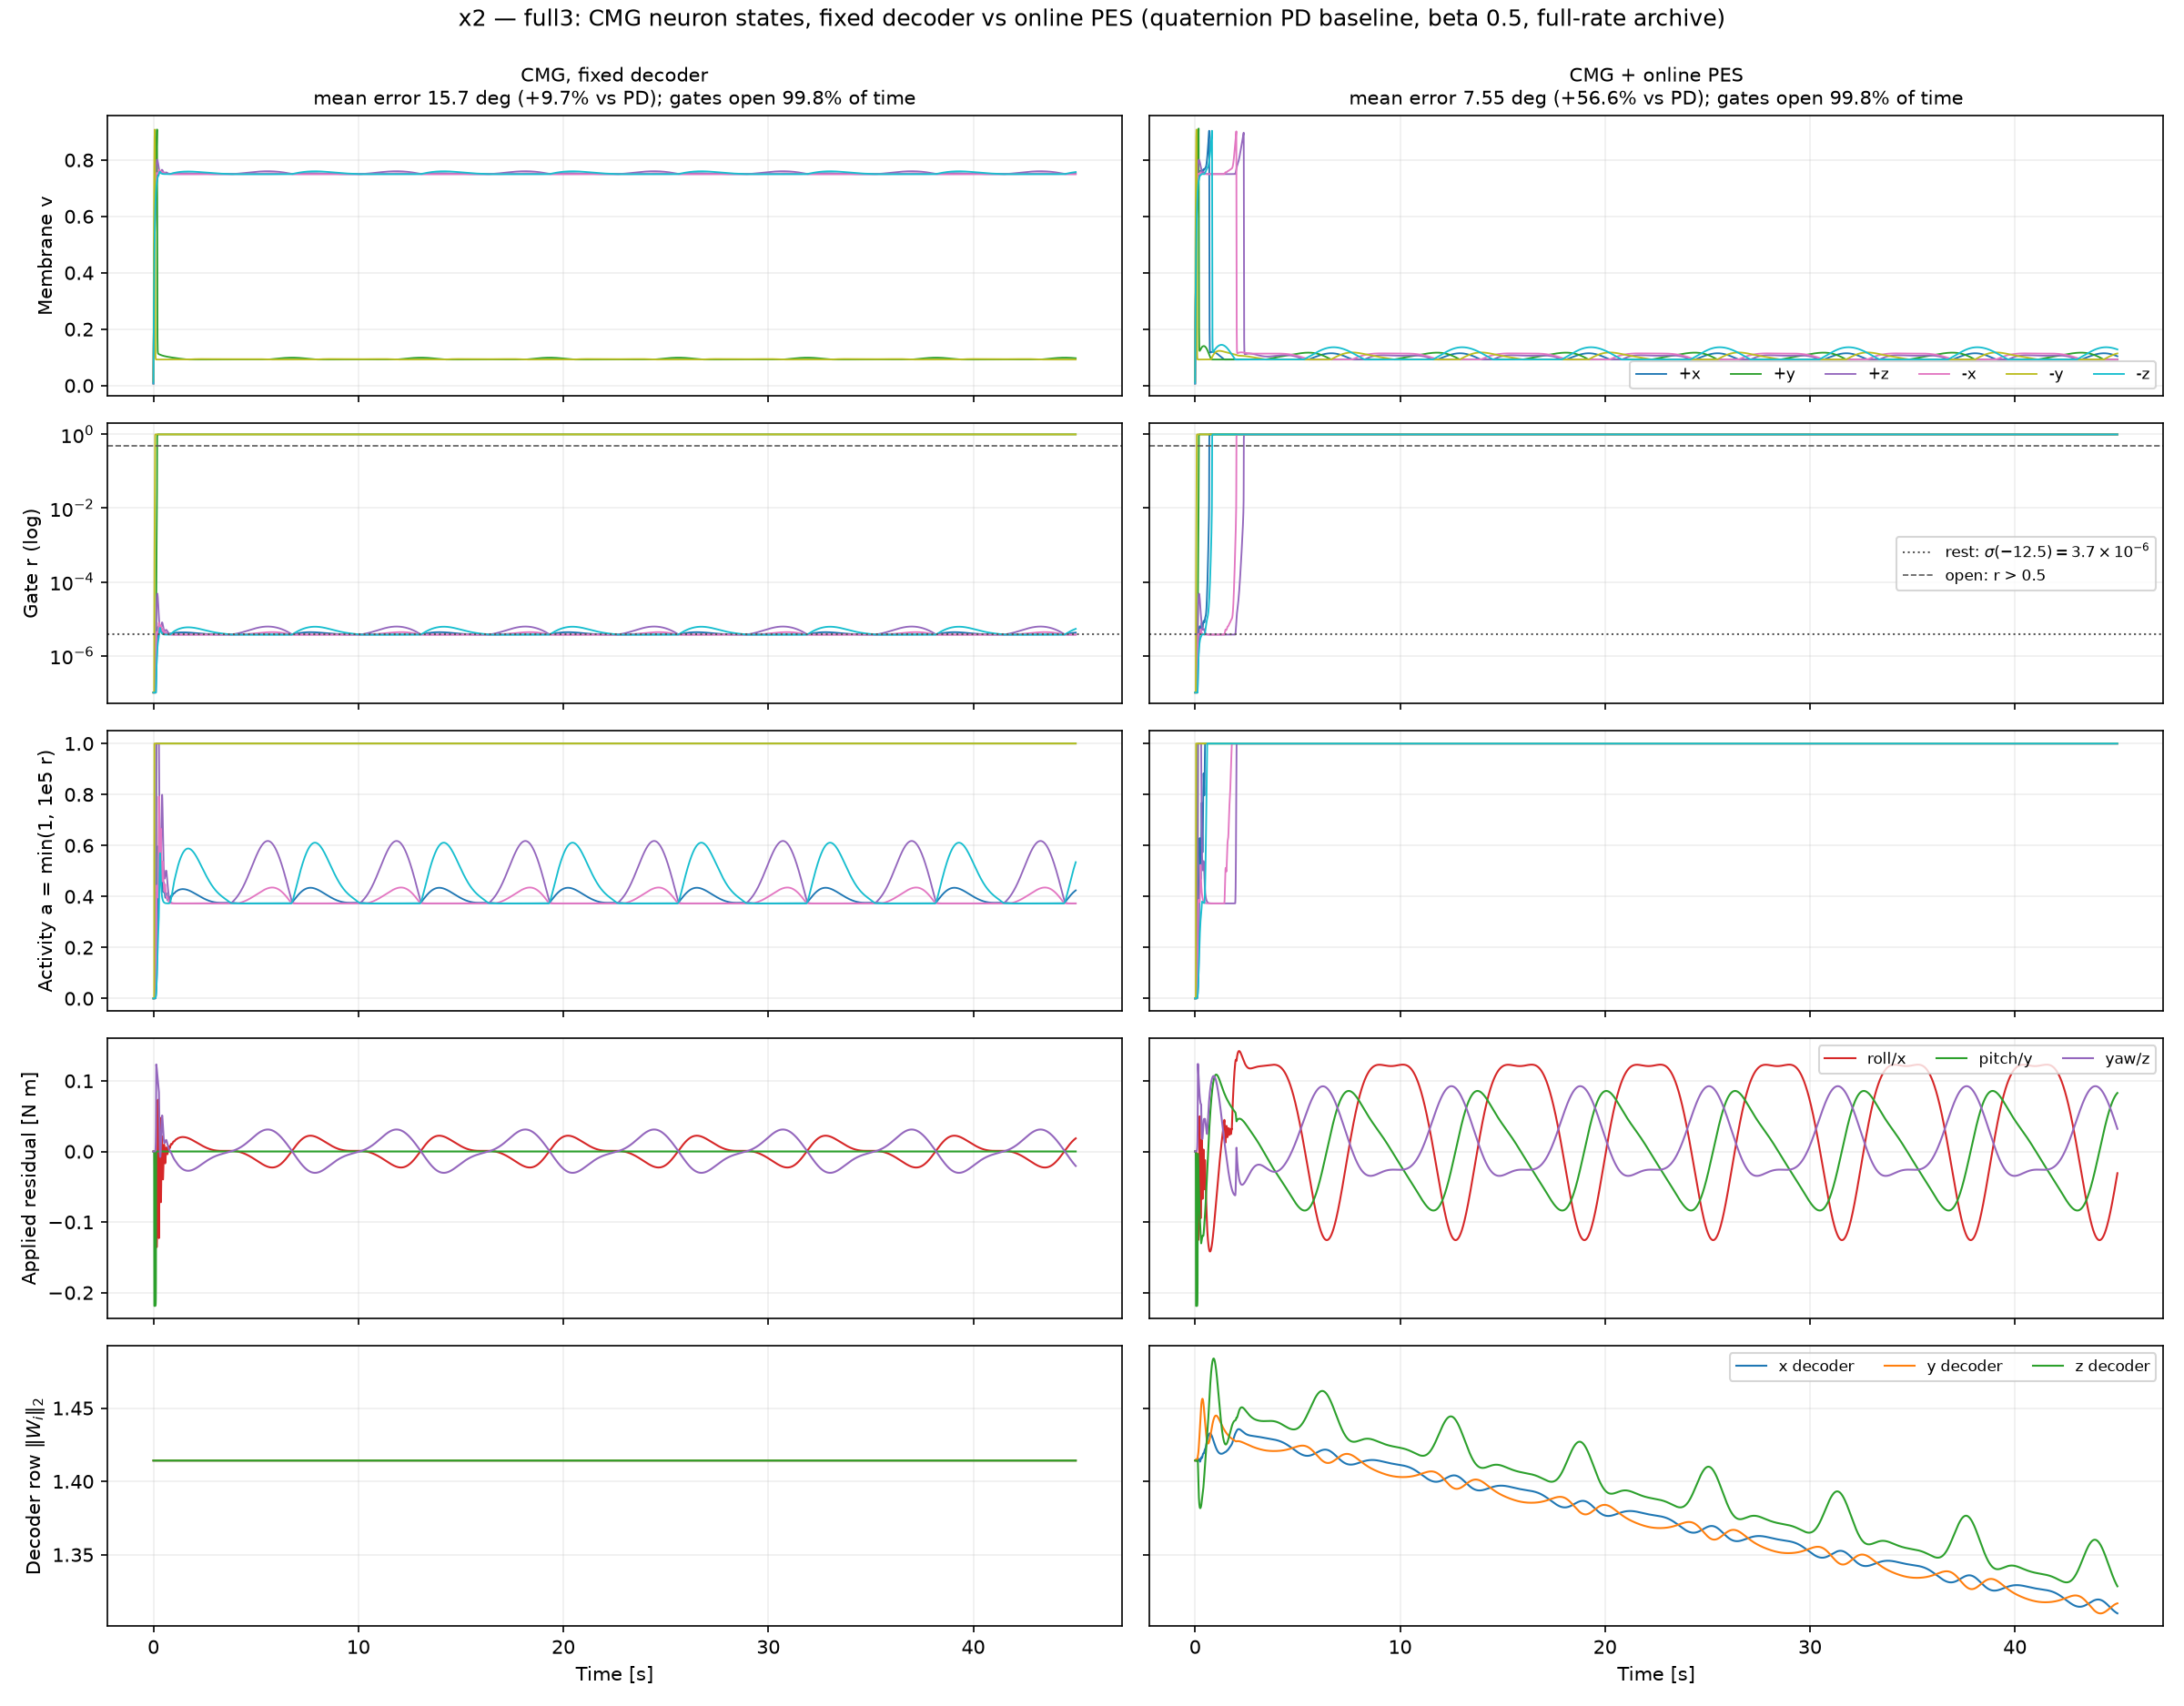
\includegraphics[width=\linewidth]{figures/09_CMGfixed_vs_CMGPES/x2_full3_fixed_vs_pes.png}
\caption{X2 Full3: internal CMG signals on the trajectory of Fig.~\ref{fig:tracking}, comparing fixed-decoder CMG (left) to online PES adaptation (right). Rows separate membrane state, raw gate $r_j$, and the clipped activity $a_j$ presented to the decoder.}
\label{fig:full3_neurons}
\end{figure*}

\subsection{Primary Five-Mission Matrix}
CMG-PES improves mean quaternion-angle tracking error in all ten nominal missions while respecting the same actuator interface as the PD baseline.
%
\begin{table}[h]
\caption{Canonical Nengo CMG--PES versus PD: mean quaternion-angle error
[rad], $45$ s, $n=1$ per cell. $S$ is the logged percentage of samples with
at least one rotor command at a bound, PD/CMG. CF2 denotes the $1.5\times$
rotor-authority design, not stock hardware.}
\label{tab:mujoco}\centering\scriptsize
\setlength{\tabcolsep}{3pt}
\begin{tabular}{llrrrr}
\toprule
Model&Mission&PD&CMG--PES&Reduction&$S$ [\%]\\\midrule
X2&Roll&.050565&.041785&17.36\%&0/0\\
&Full3&.303275&.131748&56.56\%&0/0\\
&Hard45&.294082&.138007&53.07\%&0/0\\
&Hardstep&.454528&.359355&20.94\%&.016/.239\\
&Yaw360&.075863&.029902&60.58\%&0/0\\\midrule
CF2&Roll&.051337&.042439&17.33\%&0/0\\
&Full3&.288383&.126476&56.14\%&0/0\\
&Hard45&.285449&.132319&53.65\%&0/0\\
&Hardstep&.426182&.347886&18.37\%&.137/.264\\
&Yaw360&.075812&.029870&60.60\%&0/0\\\bottomrule
\end{tabular}
\end{table}
%
The largest reductions occur on Yaw360 and Full3 and the smallest on Roll.
Hardstep has the largest absolute mean error and nonzero rotor-bound
occupancy on both models. The statistic $S$ measures post-clipping commands
near a limit, not requested-wrench infeasibility magnitude. The results
establish deterministic nominal performance relative to this fixed PD law,
not optimality over classical controllers.

Figures~\ref{fig:tracking} and \ref{fig:full3_neurons} pair tracking
performance and internal CMG signals for X2 Full3. They contrast smooth
multi-axis tracking with the corresponding neuromorphic internal dynamics.
Improvement refers to the mean metric; it need not hold at every instant.


%The primary five-mission matrix above shows that all ten cases reduce mean quaternion-angle error under CMG--PES. Gains are largest on Yaw360 and Full3 and smallest on Roll; the abrupt Hardstep case is intermediate. The reported bound-occupancy statistic detects post-clipping commands within the runner's tolerance of a limit; it is not a measure of requested-wrench infeasibility magnitude. Hardstep has small but nonzero occupancy on both models, so a blanket zero-saturation claim would be incorrect. These cases establish repeatable nominal performance; robustness to model mismatch and comparison against other baseline families are separate questions, addressed in Sec.~\ref{sec:conclusion}.

%The two featured cases bracket the matrix. Figures~\ref{fig:tracking} and \ref{fig:full3_neurons} show X2 Full3, the largest reduction that is also noise-insensitive, with the neural activity that produced it; Figs.~\ref{fig:states} and \ref{fig:cf2_hardstep_neurons} show CF2 Hardstep, the smallest reduction and the only case whose rotor commands reach a bound. Yaw360 carries the largest clean reduction but is also the most noise-sensitive entry in Table~\ref{tab:noise}, so it is reported rather than featured.

% [v8] Noise sensitivity. Generated by compile_final_sweep.py; regenerate
% from results/final_sweep_2026-09-05/compiled/table_noise.tex.
\begin{table}[ht]
\caption{Mean-error reduction versus PD under measurement noise. Entries are X2/CF2. Clean
matches the noise-free primary-matrix results; moderate is $0.010$\,rad and
$0.025$\,rad\,s$^{-1}$, realistic is $0.020$\,rad and $0.050$\,rad\,s$^{-1}$
on the attitude and rate estimates. Noisy entries average two seeds; the
seed standard deviation is given for the realistic level.}
\label{tab:noise}\centering\scriptsize
\setlength{\tabcolsep}{4pt}
\begin{tabular}{lrrr@{\,}l}
\toprule
Mission&Clean&Moderate&\multicolumn{2}{c}{Realistic}\\\midrule
Roll&17.4/17.3\%&32.3/32.4\%&32.2/32.5\%&$\pm$0.01\\
Full3&56.6/56.1\%&56.4/55.9\%&55.7/55.2\%&$\pm$0.00\\
Hard45&53.1/53.6\%&52.9/53.4\%&52.3/52.7\%&$\pm$0.01\\
Hardstep&20.9/18.4\%&20.8/18.3\%&20.6/18.1\%&$\pm$0.02\\
Yaw360&60.6/60.6\%&56.8/56.8\%&47.8/47.8\%&$\pm$0.03\\
\bottomrule
\end{tabular}
\end{table}

\begin{comment}
\begin{figure}[t]
\centering
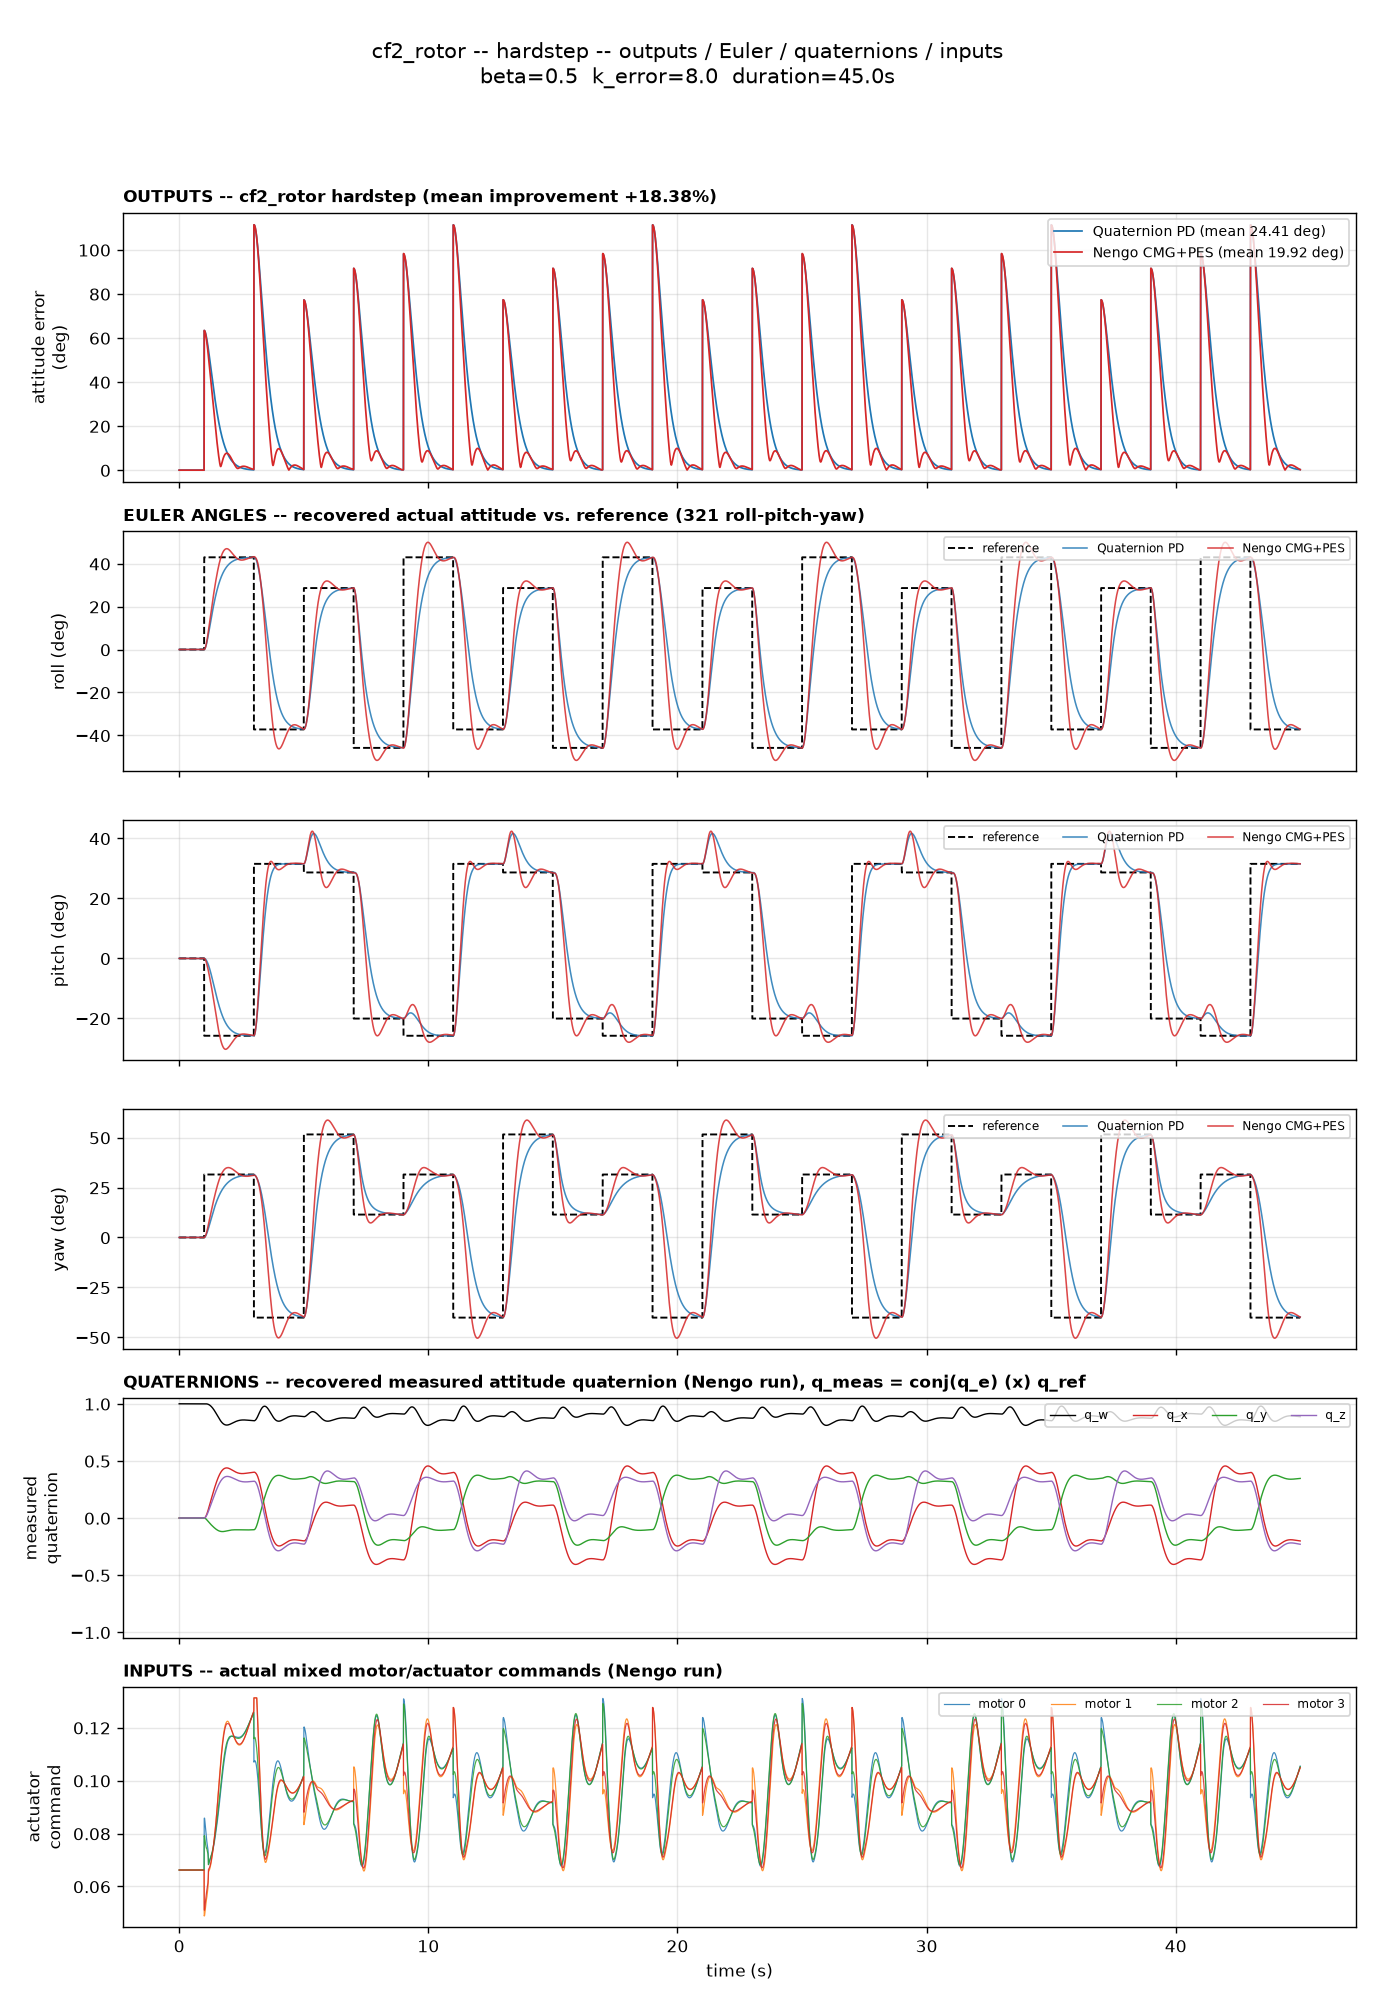
\includegraphics[width=\linewidth]{figures/02_neural_activity/attitude_detail/cf2_rotor_hardstep_attitude.png}
\caption{CF2 Hardstep mission: PD baseline versus CMG--PES augmentation on
the abrupt step reference. This is the hardest case in the matrix, the
smallest reduction ($18.4\%$), and the only one whose rotor commands reach a
bound ($S=.137/.264$). The residual stays inside its
authority envelope and the augmented loop remains better than the baseline
throughout.}
\label{fig:states}
\end{figure}
\end{comment}

%%%%%%%%%%%%%%%%%%%%%%%%%%%%%%%%%%%%%%%%%%%%%%%%
\subsection{Sensitivity to Measurement Noise}
\label{sec:noise}

Each of the ten cases was rerun at two synthetic noise levels and two
paired seeds. At every step, independent zero-mean Gaussian samples form
a small Euler-angle quaternion left-multiplied into $q$, and additive
Gaussian samples corrupt each angular-rate component. These levels are
not calibrated sensor specifications. Crucially, the runner evaluates
$\theta_q$ from the \emph{corrupted} quaternion used by the controller,
not from an independent ground-truth attitude. Table~\ref{tab:noise}
therefore measures noisy-feedback error.

All reported noisy-feedback reductions remain positive. At the higher
level they range from $18.08$ to $55.75\%$; Yaw360 loses about 12.8 pp
relative to clean feedback, whereas Roll's relative reduction increases.
Sample SD ranges are $.001$--$.101$ pp at low noise and $.002$--$.031$ pp
at high noise. Two seeds demonstrate limited repeatability, not a reliable
population confidence interval or effectively deterministic behavior.

\begin{comment}
\begin{figure}[t]
\centering
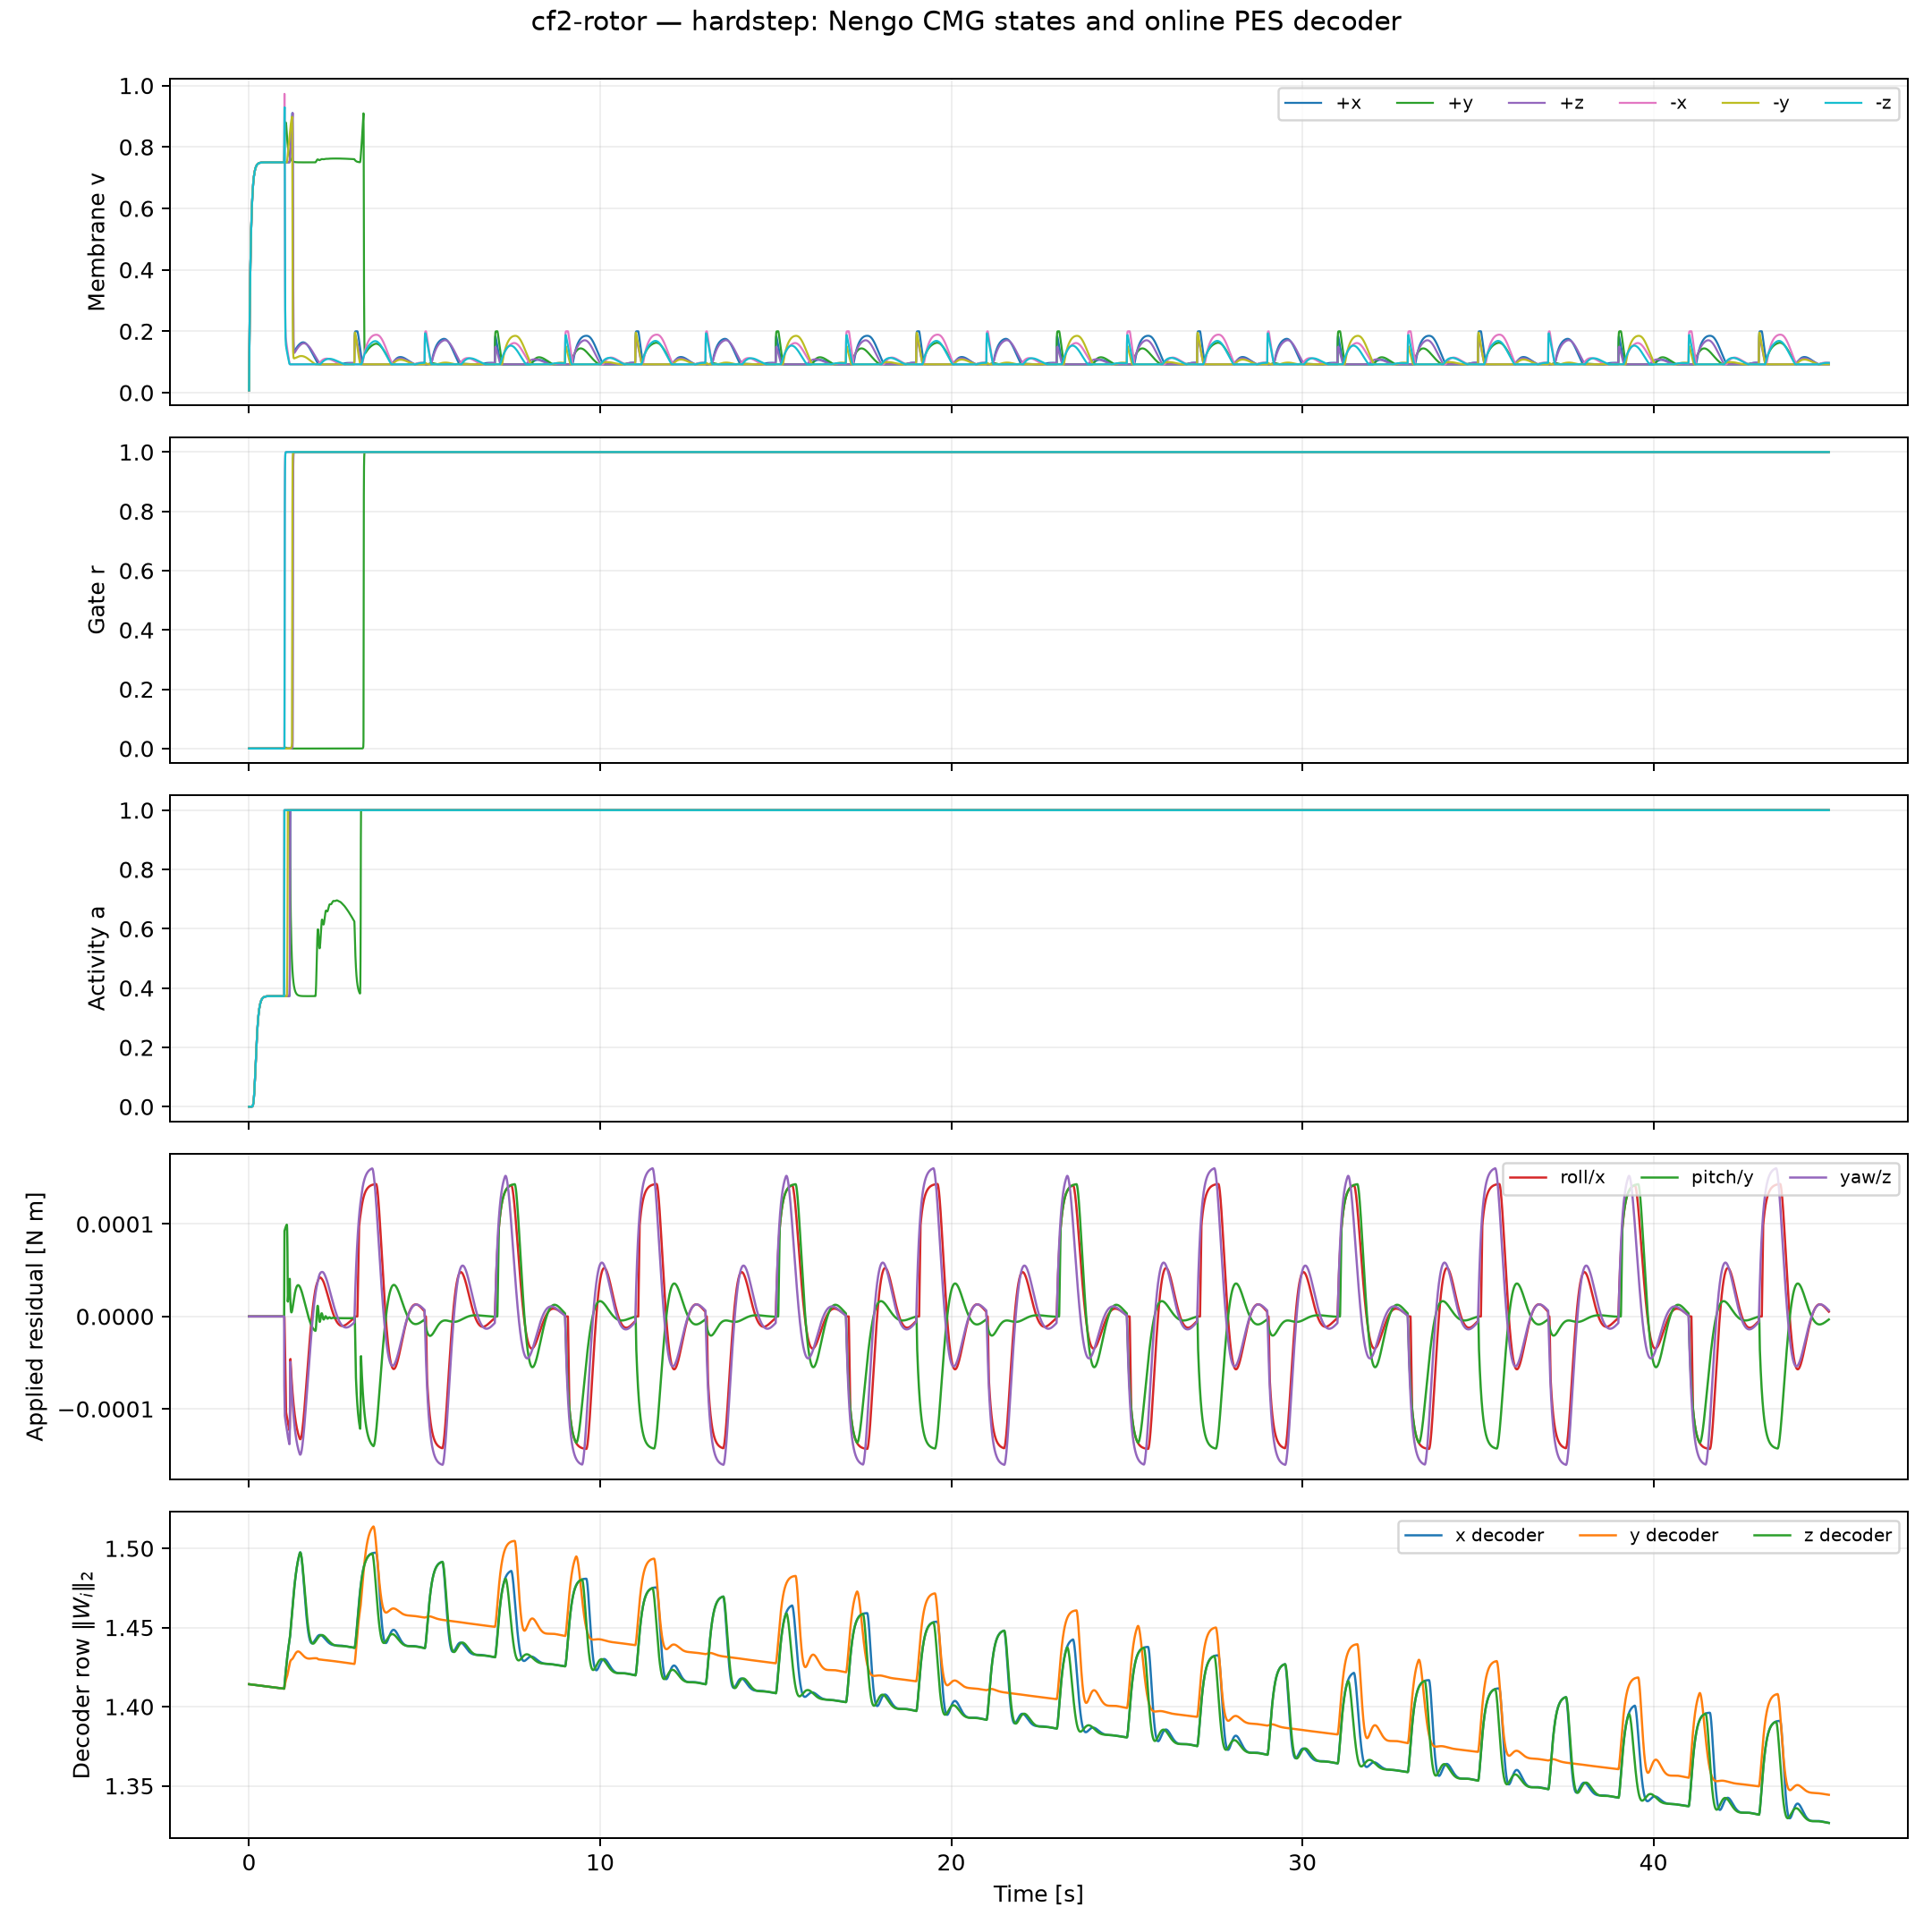
\includegraphics[width=\linewidth]{figures/02_neural_activity/cf2-rotor_hardstep_neurons.png}
\caption{CF2 Hardstep: internal CMG signals on the same trajectory as
Fig.~\ref{fig:states}. The plot separates membrane state, raw gate $r_j$, and
the clipped activity $a_j=\clip_{[0,1]}(Gr_j)$ presented to the decoder,
illustrating the readout saturation of Sec.~IV-D under the one mission that
also drives the rotors to a bound.}
\label{fig:cf2_hardstep_neurons}
\end{figure}
\end{comment}

%%%%%%%%%%%%%%%%%%%%%%%%%%%%%%%%%%%%%%%
\subsection{Ablation: What Drives the Improvement?}\label{sec:ablation}

We distinguish decoder adaptation (PES), input-dependent conductance modulation ($\chi$), and readout gain ($G$). Toggling $\chi$ retains the base shunting term $g_0r_j^2$; it is not removal of all conductance or all CMG dynamics.
Fixed-decoder residuals already improve some missions: in the audited direct
X2 runs their mean reductions range from about 0.12\% to 10.27\%; the
corresponding CF2-design range is 0.06\% to 6.80\%. Thus it is inaccurate
to say that fixing the decoder removes \emph{all} improvement. PES produces
the much larger 17.3--60.6\% primary reductions. Separately, toggling
$\chi$ with the decoder mode held fixed is numerically indistinguishable
under the tested settings. Decoder adaptation is therefore the principal lever in the tested regime.

%Readout saturation does not imply negligible conductance. In the fresh canonical X2 Full3 rerun, $r_j>0.9$ for $97.7\%$ of unit-samples and mean $c_j\tau$ is $7.08$. Yet $a_j$ clips at $r_j=10^{-5}$.
%Moreover, with $\gamma=2$ and $v_j\ge0$, $r_j\ge1/2$ implies $b_j\ge1/2$ in \eqref{eq:gate_step}; its convex update preserves that high-gate region. Conductance can therefore change membrane voltage without producing a distinguishable decoded activity.

%The resulting decoder has a useful exact reduction. On an interval with
%$\bm a_k=\bar{\bm a}$ and inactive weight projection, let
%$\bm z_k=W_k\bar{\bm a}$. Then \eqref{eq:pes} gives
%\begin{equation}
% \bm z_{k+1}=(1-\lambda_W)\bm z_k+
% \eta\|\bar{\bm a}\|^2[\bm y_k^*-\clip_{[-1,1]}(\bm z_k)].
% \label{eq:constantbasis}
%\end{equation}
%When readout clipping is inactive, this is a first-order target filter.
%For six unit activities its pole is $.995199$, corresponding to about
%$.104$ s. This is a direct-backend identity under the stated conditions,
%not equivalence of the full transient CMG or delayed Nengo dynamics.
%The recorded X2 Full3 activity is identically one after $2.02$ s; the
%reduced recursion matches its saved decoder to $8\times10^{-16}$.

%A focused direct-backend sweep uses $G\in\{1,10^3,10^5,10^6\}$ and $\chi\in\{0,1\}$ on X2 Full3 and CF2 Hardstep. Their reductions remain $56.04$--$56.97\%$ and $18.34$--$18.46\%$, respectively. In contrast, X2 Roll ranges from effectively zero at $G=1$ to $17.36\%$ at $10^5$ and $57.76\%$ at $10^6$ (also tested at $10^2,10^4$). These are fixed-$\eta$ sensitivity tests: before clipping, same-feature PES excitation scales as $\eta G^2\|\bm r\|^2$. They do not isolate neuron expressiveness. Eight selected Nengo checks agree with the direct mean errors to relative difference $1.13\times10^{-7}$.

%\begin{table}[ht]
%\centering\footnotesize
%\caption{Direct-backend controls: mean-error reduction over matched
%PD [\%]. Same $W_0$, PES teacher/update, leak, caps, and allocation;
%canonical CMG uses $G=10^5$. One deterministic run per cell.}
%\label{tab:simplebasis}
%\setlength{\tabcolsep}{4pt}
%\begin{tabular}{lrrr}
%\toprule
%Case & CMG & Paired-linear & Constant\\\midrule
%X2 Roll &17.36&0.73&57.78\\
%X2 Full3 &56.56&6.70&56.98\\
%CF2 Hardstep &18.37&1.50&18.38\\\bottomrule
%\end{tabular}
%\end{table}

\begin{figure}[ht]
\centering
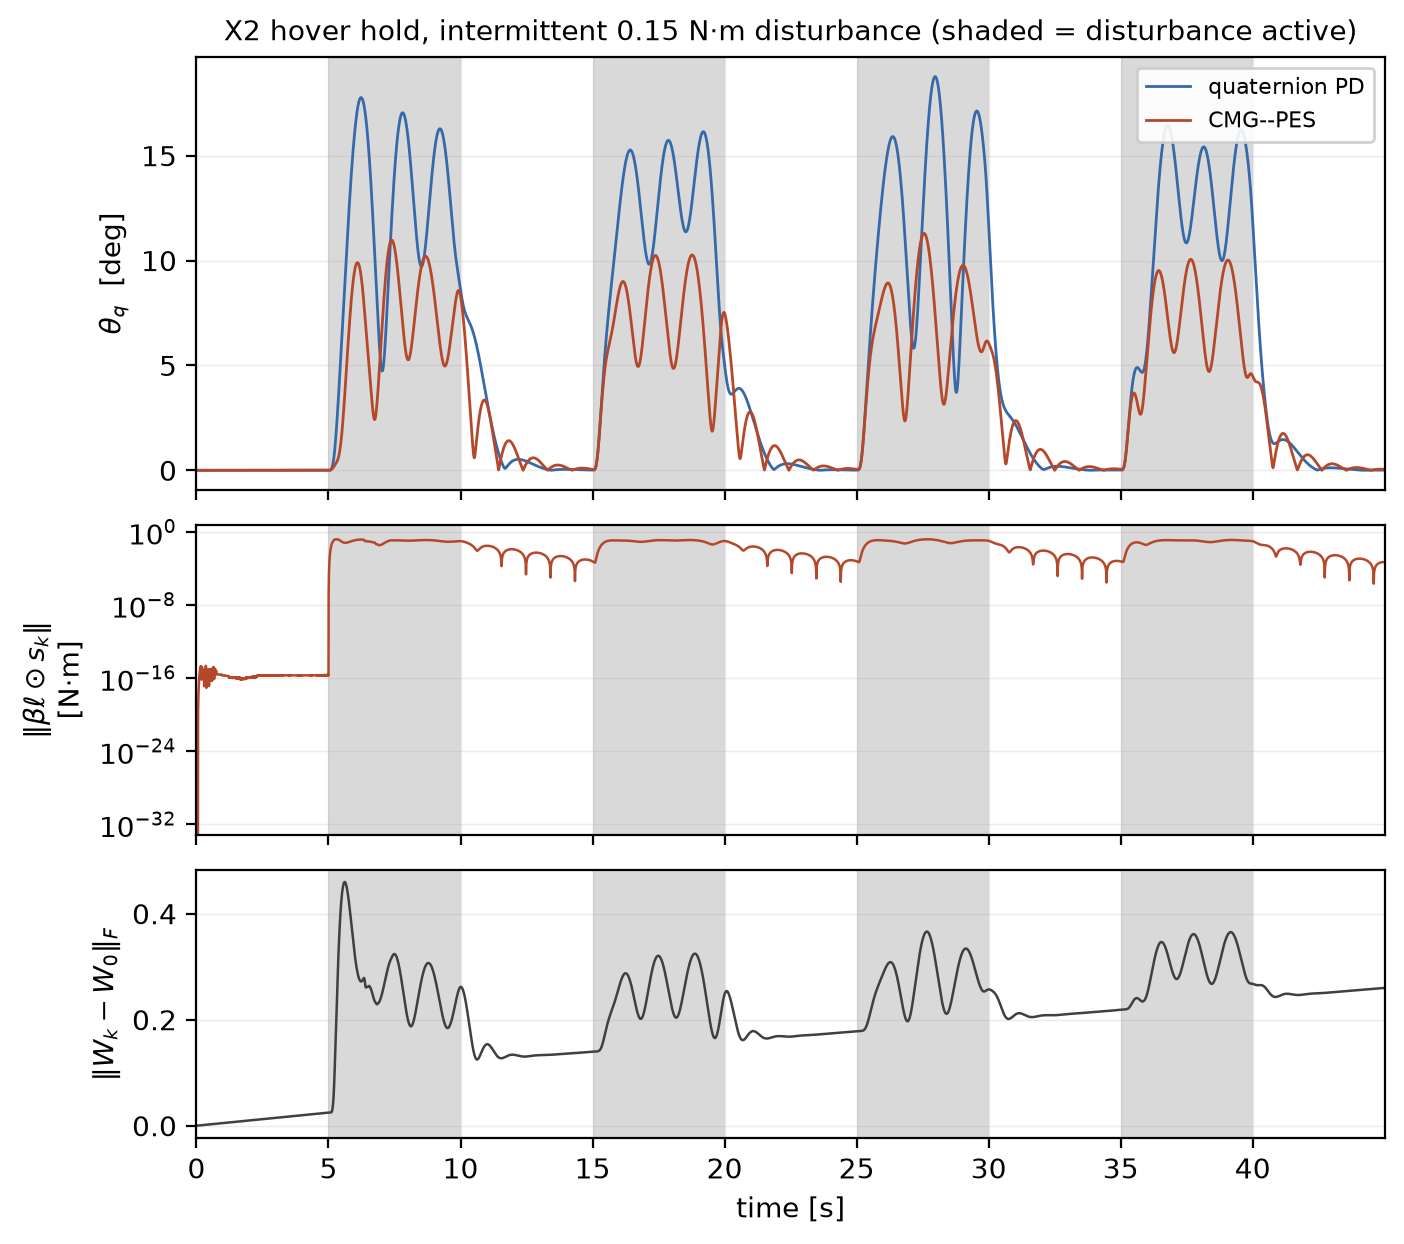
\includegraphics[width=\linewidth]{figures/07_disturbance_and_noise/hover_intermittent.png}
\caption{X2 hover hold under four $0.15$\,N\,m disturbance bursts (shaded)
separated by quiet intervals. Top: attitude error. Centre: residual
magnitude, logarithmic. Bottom: decoder displacement from $W_0$. The
residual is at numerical precision before the first burst. This means
negligible initial correction, not zero computation or energy cost.}
\label{fig:hover_int}
\end{figure}

%%%%%%%%%%%%%%%%%%%%%%%%%%%%%%%%%%%%%%%%%%%%%%%%%%%%%%%%
\subsection{Disturbance Rejection and Retention}
\label{sec:disturbance}
An equilibrium test applies
$\bm\tau_{\rm d}=d_b\rho(t)[\sin(1.31t+.2),\allowbreak
.8\sin(1.73t+1.1),\allowbreak.6\sin(2.17t+2)]\T$ in body axes.
After 5 s of quiet, $\rho$ alternates 5-s on/off intervals with 0.25-s
raised-cosine edge ramps. For X2, $d_b=.15$ N\,m: the first component's
amplitude is .15 N\,m, not a bound on the vector norm.
The four-burst 45-s experiment in Fig.~\ref{fig:hover_int} reduces
burst-phase mean error from $11.50^\circ$ to $6.65^\circ$ ($42.2\%$),
and post-burst quiet error from $1.21^\circ$ to $.99^\circ$ ($18.0\%$).
The corrected CF2 rerun uses $d_b=.00015$ N\,m, a selected scaling rather
than an exact inertia-ratio match; its full-run mean falls from
$.141199$ to $.070259$ rad ($50.24\%$).

%The 180-s X2 record contains eighteen bursts and seventeen complete post-burst quiet intervals, not sixteen bursts. Decoder displacement reaches $.797$ at the final sample, with maximum absolute weight $1.089$.
%One quiet interval is about $4\%$ worse than PD. Continued weight change and nonzero quiet-phase errors do not establish convergence. Because learning and leakage remain active, and the multi-sine phase is not reset between bursts, this study shows persistent adaptation, not causal proof of reuse without relearning. A reset-decoder or frozen-decoder control is needed to test that hypothesis.

\subsection{Neuron-Family Comparison}
Across neuron models, improved tracking typically requires greater residual effort; CMG--PES lies near a favorable point on this effort--accuracy tradeoff.
The Nengo benchmark contains two models, five missions, and eleven controllers: PD and fixed/PES variants of CMG, LIF, ALIF, Izhikevich \cite{izhikevich2003}, and LIFRate. All share the same bounded residual, saturation, and allocation interface; only the neuron dynamics and the mapping from native state to activity differ.

Figure~\ref{fig:mech_dashboard} summarizes the full matrix on both
platforms: mean tracking error and realized residual effort for every
family and learning mode. Two consistent patterns emerge. First, PES adaptation is the dominant lever across families: fixed
decoders rarely match their PES counterparts, even when the underlying
neuron dynamics are more expressive. Second, lower error does not come for
free. Some Izhikevich--PES cells achieve the smallest mean error, but the
audit reports a substantially larger average normalized residual RMS
(approximately 0.37 versus 0.12 for CMG--PES) and larger decoder movement,
so equal output caps do not imply equal realized correction effort.

Sparse LIF/ALIF activity in some cells limits the effective feature basis at
the tested operating point, which can blunt online learning without
implying that those families cannot learn under different encodings or gain
settings. The supported conclusion is therefore a tracking--effort tradeoff:
CMG--PES attains comparable tracking at markedly lower realized residual
effort and more conservative decoder motion in this benchmark.

In Fig.~\ref{fig:full3_neurons}, gate/activity saturation and rotor
clipping are distinct phenomena. Labels referring to a residual torque
denote the requested difference $\bm\delta$, not its post-allocation effect.

% [v10] One two-column figure replaces the two single-column dashboards.
% The 181 mm source was previously scaled into an 88 mm column, a 2.05x
% reduction that left its labels near 3 pt. Drawn at 1:1 here.
\begin{figure*}[h]
    \centering
    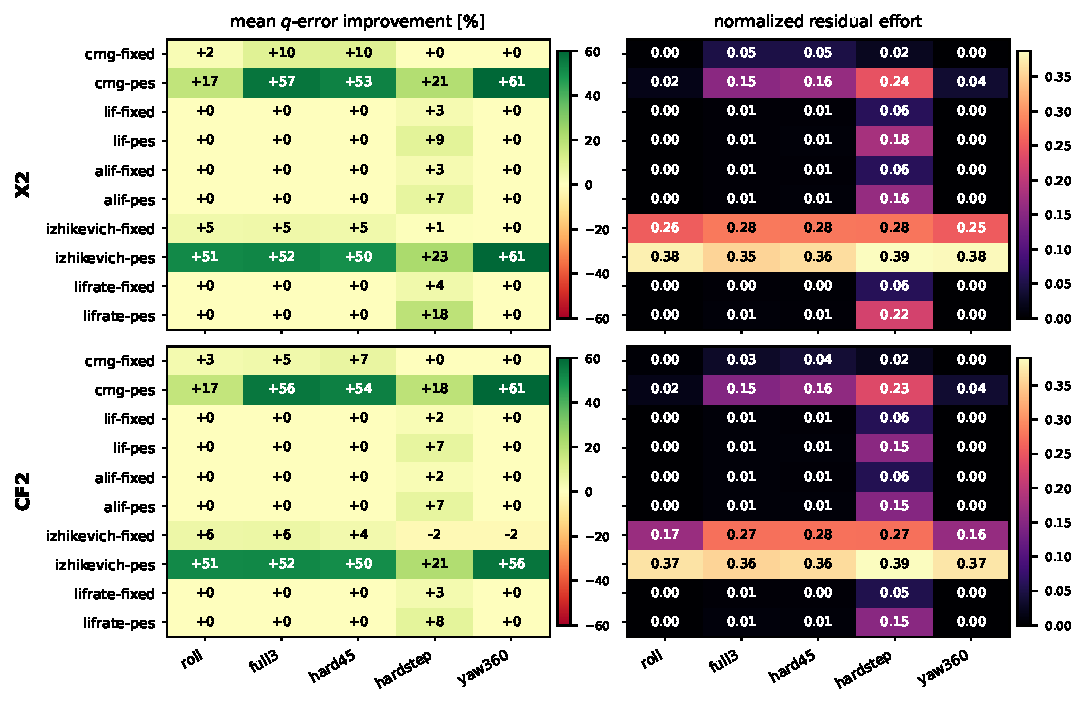
\includegraphics[width=\textwidth]{figures/08_Nengo_neuron_family/mechanism_both_platforms.pdf}
    \caption{Mechanism separation across the Nengo neuron-family benchmark,
    X2 (top) and CF2 (bottom). Left: mean $q$-error improvement over the PD
    baseline. Right: normalized residual effort, the RMS residual as a
    fraction of the per-axis limit. Rows are neuron family and learning
    mode, columns are missions; every cell uses the same bounded residual,
    saturation, and allocation interface. Two patterns hold on both
    platforms: PES adaptation, not the neuron model, separates the improving
    rows from the flat ones; and the families that match or exceed
    CMG--PES on error do so at three to twenty times its residual effort.}
    \label{fig:mech_dashboard}
\end{figure*}

\section{Discussion and Conclusion}
\label{sec:conclusion}
% [v7] Rewritten: states the positive result once and plainly, keeps the
% limits in one place instead of after every sentence, and separates the
% analog outlook from the claims.
A bounded neuromorphic residual can augment a fixed quaternion PD baseline without changing its gains or actuator interface. Using six continuous CMG units with eighteen PES-adapted decoder weights, the augmented loop reduces mean quaternion-angle tracking error by $17.3$--$60.6\%$ over ten matched 45-s MuJoCo cases on two modeled platforms, while respecting rotor saturation and recovering the baseline exactly at zero residual authority. Direct and Nengo realizations agree to $2.013\times10^{-6}$ relative mean error.

Mechanism studies show that, in the tested regime, decoder adaptation is the dominant source of improvement: fixed-decoder residuals yield only modest reductions, and toggling the input-dependent conductance term ($\chi$) with the decoder mode held fixed is numerically indistinguishable. Across CMG, LIF/ALIF, Izhikevich, and LIFRate bases, PES is the consistent differentiator, while neuron dynamics mainly set an effort--accuracy tradeoff (matching error often requires substantially more residual effort). The observed readout saturation $a_j=\clip(Gr_j,0,1)$ suggests $G$ is a key sensitivity parameter.

Limitations: results are in simulation (Sec.~\ref{sec:noise} bounds noise sensitivity, but model mismatch and hardware effects are not addressed); the repeated-disturbance retention horizon is limited; and bounded commands, states, and weights are implementation properties rather than closed-loop stability proofs.

Future work will include integral-action baselines, matched-effort comparisons against non-neural bounded bases, systematic sweeps of $G$ and $\chi$, longer-horizon retention studies, held-out evaluations with frozen learned weights, extension to full 6-DOF systems, and, most importantly, validation on physical robotic platforms, including aerial, ground, and other dynamical systems. The same bounded-residual wrapper can also be extended to nonlinear and optimal-control baselines subject to hard actuator constraints.



% Finalize human authors, affiliations, funding, and any required tool-use
% disclosure before submission. No invented author identities are supplied.
\bibliographystyle{IEEEtran}
\bibliography{references}
\end{document}
